
%%%% Bachelor Research Assignemt in Argument Mining
%%%% by Klio Fragkedaki

%----------------------------------------------------------------------------------------
%	PACKAGES AND OTHER DOCUMENT CONFIGURATIONS
%----------------------------------------------------------------------------------------

\documentclass[
11pt, % The default document font size, options: 10pt, 11pt, 12pt
%oneside, % Two side (alternating margins) for binding by default, uncomment to switch to one side
english,
singlespacing, % Single line spacing, alternatives: onehalfspacing or doublespacing
%draft, % Uncomment to enable draft mode (no pictures, no links, overfull hboxes indicated)
%nolistspacing, % If the document is onehalfspacing or doublespacing, uncomment this to set spacing in lists to single
%liststotoc, % Uncomment to add the list of figures/tables/etc to the table of contents
%toctotoc, % Uncomment to add the main table of contents to the table of contents
%parskip, % Uncomment to add space between paragraphs
%nohyperref, % Uncomment to not load the hyperref package
headsepline, % Uncomment to get a line under the header
%chapterinoneline, % Uncomment to place the chapter title next to the number on one line
%consistentlayout, % Uncomment to change the layout of the declaration, abstract and acknowledgements pages to match the default layout
]{BachelorAssignment} % The class file specifying the document structure
\usepackage[utf8]{inputenc} % Required for inputting international characters
\usepackage[T1]{fontenc} % Output font encoding for international characters

\usepackage{mathpazo} % Use the Palatino font by default
\usepackage{listings} % code in Appendix
\usepackage{verbatimbox}

\usepackage{color}
\definecolor{light-gray}{gray}{0.85}

\usepackage[backend=bibtex,style=authoryear,natbib=true]{biblatex} % Use the bibtex backend with the authoryear citation style (which resembles APA)

\addbibresource{example.bib} % The filename of the bibliography

\usepackage[autostyle=true]{csquotes} % Required to generate language-dependent quotes in the bibliography
\usepackage[titles]{tocloft}

\usepackage{wrapfig}
\usepackage{subfig}
\usepackage{float}
\usepackage{amsmath}
\usepackage{xcolor}
%----------------------------------------------------------------------------------------
%	MARGIN SETTINGS
%----------------------------------------------------------------------------------------

\definecolor{maroon}{cmyk}{0,0.87,0.68,0.32}
\definecolor{halfgray}{gray}{0.55}
\definecolor{ipythonFrame}{RGB}{207,207,207}
\definecolor{ipythonBg}{RGB}{247,247,247}
\definecolor{ipythonRed}{RGB}{186,33,33}
\definecolor{ipythonGreen}{RGB}{0,128,0}
\definecolor{ipythonCyan}{RGB}{64,128,128}
\definecolor{ipythonPurple}{RGB}{170,34,255}

\geometry{
	paper=a4paper, % Change to letterpaper for US letter
	inner=2.8cm, % Inner margin
	outer=2.8cm, % Outer margin
	%bindingoffset=.5cm, % Binding offset
	top=1.5cm, % Top margin
	bottom=1.5cm, % Bottom margin
	%showframe, % Uncomment to show how the type block is set on the page
}

\newcommand*{\enableboldchapterintoc}{%
	\addtocontents{toc}{\string\renewcommand{\protect\cftchapfont}{\protect\normalfont\protect\bfseries}}
	\addtocontents{toc}{\string\renewcommand{\protect\cftchappagefont}{\protect\normalfont\protect\bfseries}}
	\addtocontents{toc}{\string\renewcommand{\protect\cftchapleader}{\protect\bfseries\protect\cftdotfill{\protect\cftsecdotsep}}}% dot leaders in bold
}

\newcommand*{\disableboldchapterintoc}{%
	\addtocontents{toc}{\string\renewcommand{\protect\cftchappagefont}{\protect\normalfont}}
	\addtocontents{toc}{\string\renewcommand{\protect\cftchapfont}{\protect\normalfont}}
	\addtocontents{toc}{\string\renewcommand{\protect\cftchapleader}{\protect\normalfont\protect\cftdotfill{\protect\cftsecdotsep}}}% 
}

\lstdefinelanguage{iPython}{
	morekeywords={access,and,break,class,continue,def,del,elif,else,except,exec,finally,for,from,global,if,import,in,is,lambda,not,or,pass,print,raise,return,try,while},%
	%
	sensitive=true,
	morecomment=[l]\#,
	morestring=[b]',
	morestring=[b]",
	%
	morestring=[s]{'''}{'''},% used for documentation text (mulitiline strings)
	morestring=[s]{"""}{"""},
	%
	literate=*{=}{{\textcolor{ipythonPurple}{=}}}{1}
	{+}{{\textcolor{ipythonPurple}{+}}}{1}
	{*}{{\textcolor{ipythonPurple}{*}}}{1}
	{/}{{\textcolor{ipythonPurple}{/}}}{1}
	{-}{{\textcolor{ipythonPurple}{-}}}{1}
	{?}{{\textcolor{ipythonPurple}{?}}}{1},
	%
	%
	identifierstyle=\color{black}\ttfamily,
	commentstyle=\color{ipythonCyan}\ttfamily,
	stringstyle=\color{ipythonRed}\ttfamily,
	keepspaces=true,
	showspaces=false,
	showstringspaces=false,
	%
	rulecolor=\color{ipythonFrame},
	frame=single,
	frameround={t}{t}{t}{t},
	framexleftmargin=6mm,
	numbers=left,
	numberstyle=\tiny\color{halfgray},
	%
	backgroundcolor=\color{ipythonBg},
	basicstyle=\scriptsize,
	keywordstyle=\color{ipythonGreen}\ttfamily,
}

\lstset{
	breaklines=true,
	identifierstyle=\color{black}\ttfamily,
	basicstyle=\scriptsize,
	backgroundcolor=\color{light-gray},
	tabsize=2,
}


%----------------------------------------------------------------------------------------
%	THESIS INFORMATION
%----------------------------------------------------------------------------------------

\thesistitle{Argument Mining}
\supervisor{Prof. Panagiotis Louridas}
\examiner{} % Your examiner's name, this is not currently used anywhere in the template, print it elsewhere with \examname
\author{Klio Fragkedaki} % Your name, this is used in the title page and abstract, print it elsewhere with \authorname
\addresses{} % Your address, this is not currently used anywhere in the template, print it elsewhere with \addressname

\subject{Natural Language Processing} % this is not currently used anywhere in the template, print it elsewhere with \subjectname
\keywords{} % Keywords for your thesis, this is not currently used anywhere in the template, print it elsewhere with \keywordnames
\university{\href{https://aueb.gr/}{Athens University of Economics and Business}}
\department{\href{https://my.dmst.aueb.gr/}{Department of Management Science and Technology}} % Your department's name and URL, this is used in the title page and abstract, print it elsewhere with \deptname

\AtBeginDocument{
\hypersetup{pdftitle=\ttitle} % Set the PDF's title to your title
\hypersetup{pdfauthor=\authorname} % Set the PDF's author to your name
\hypersetup{pdfkeywords=\keywordnames} % Set the PDF's keywords to your keywords
}

\begin{document}

\frontmatter % Use roman page numbering style (i, ii, iii, iv...) for the pre-content pages

\pagestyle{plain} % Default to the plain heading style until the thesis style is called for the body content

%----------------------------------------------------------------------------------------
%	TITLE PAGE
%----------------------------------------------------------------------------------------

\begin{titlepage}
\begin{center}

\vspace*{.06\textheight}
{\scshape\LARGE \univname\par}\vspace{1.5cm}
\textsc{\Large Bachelor Research Assignment}\\[0.5cm]

\HRule \\[0.4cm]
{\huge \bfseries \ttitle\par}\vspace{0.4cm}
\HRule \\[1.5cm]
 
\begin{minipage}[t]{0.4\textwidth}
\begin{flushleft} \large
\emph{Author:}\\
{\authorname} 
\end{flushleft}
\end{minipage}
\begin{minipage}[t]{0.4\textwidth}
\begin{flushright} \large
\emph{Supervisor:} \\
{\supname} 
\end{flushright}
\end{minipage}\\[3cm]
 
\vfill

\large \textit{An assignment submitted as part of\\ Bachelor degree}\\[0.3cm]
\textit{in the}\\[0.4cm]
\deptname\\[2cm]
 
\vfill
\vspace{5cm}

{\large \today}\\[4cm] % Date
%\includegraphics{Logo} % University/department logo
 
\end{center}
\end{titlepage}

%----------------------------------------------------------------------------------------
%	LIST OF CONTENTS/FIGURES/TABLES PAGES
%----------------------------------------------------------------------------------------

\tableofcontents % Prints the main table of contents

%----------------------------------------------------------------------------------------
%	ACKNOWLEDGEMENTS
%----------------------------------------------------------------------------------------

\section*{Acknowledgments}
	I would like to thank Vasiliki Efstathiou for being the second annotator and a great supervisor, as well as my Professor Panos Louridas.

%----------------------------------------------------------------------------------------
%	ABBREVIATIONS
%----------------------------------------------------------------------------------------

\begin{abbreviations}{ll}

\textbf{SVM}  & \textbf{S}upport \textbf{V}ector \textbf{M}achine\\
\textbf{LR}   & \textbf{L}ogistic \textbf{R}egression\\
\textbf{NB}   & \textbf{N}aive \textbf{B}ayes classifier\\
\textbf{RF}   & \textbf{R}andom \textbf{F}orest\\
\textbf{RNN}  & \textbf{R}ecurrent \textbf{N}eural \textbf{N}etworks for Language Models\\
\textbf{RF}   & \textbf{R}andom \textbf{F}orest\\
\textbf{CRF}  & \textbf{C}onditional \textbf{R}andom \textbf{F}orest\\
\textbf{ML}	  & \textbf{M}aximum \textbf{L}ikelihood\\
\textbf{TES}  & \textbf{T}extual \textbf{E}ntailment \textbf{S}uites\\
\textbf{P}    & \textbf{P}arsing Using a Context-Free Grammar\\
\textbf{LSTM} & \textbf{L}ong \textbf{S}hort-\textbf{t}erm \textbf{M}emory\\
\textbf{POS} & \textbf{P}art \textbf{O}f \textbf{S}peech\\

\end{abbreviations}

%----------------------------------------------------------------------------------------
%	RESEARCH CONTENT - CHAPTERS
%----------------------------------------------------------------------------------------

\mainmatter

\pagestyle{thesis}


\chapter{Introduction}

\label{Chapter1}

\section{Definition} 

Argument mining is a relatively new research field in natural language processing. The aim of this research is the auto detection and identification of argumentative structures expressed in text. In order to perform extraction and evaluation of arguments, computer science and artificial intelligence is used. \par

An argument is a group of premises conducted to support a claim (\cite{Palau2009}). When it comes to real world, arguments are hardly identified even by experts (\cite{Lippi2015}). The ambiguity of natural language, the implicit content, the different ways of expressing and the complex structure of arguments are the main reasons why argument mining is a challenging research field. Labeled corpora are scarce which is a fact that slows down field's potential growth (\cite{Lippi2015}). \par

The purpose of argument mining is to understand what kind of views have been expressed in the examined text and why they are held. Argument mining has derived from opinion mining and sentiment analysis  research area, in which the only goal is to understand the opinions about a certain topic (\cite{Lawrence2015}). \par

\section{Research Goal}
 My research goal is to identify argumentative statements by using two different approaches; the structural approach which is based on hand coded rules and the statistical approach, which based on supervised and deep learning algorithms. \par
 
 The structural approach uses lexical cues that have been identified by linguists as signs of argumentative speech. As an example, words such as "because", "therefore", "in order to" are common cues of arguments. However, these argumentative patterns are rarely used in practice,	since human discourse involves a lot of information which is being implied rather than being explicitly stated. \par
 
 On the other hand, the statistical approach relies on examples of pieces of text that have been manually labeled as argumentative or non-argumentative. These are used for training models in order to automatically identify arguments in free text without the use of predefined lexical cues and rules. The challenging part is the construction of a manually annotated data-set, given the fact that a large amount of data are required for training such models. \par
 
 The fundamental research questions that will be addressed in this assignment are the following:
 \begin{itemize}
   \item To what extent are the lexical rules drafted by a structural approach capable of successfully identifying arguments in existing resources of labeled data?
   \item Do the statistical approaches outperform these results?
 \end{itemize}  


\section{Assignment's Structure}

This paper of research is organized into 6 chapters. Chapter \ref{Chapter2} presents the state of the art in argument mining, and introduces the two different approaches; the structural and the machine learning approach. Chapters \ref{Chapter3} and \ref{Chapter4} describe in detail the methods and results of both approaches implemented in the scope of this study. Chapter \ref{Chapter5} contains the corpora created for the supervised algorithm, while chapter \ref{Chapter6} concludes with a look to future work. \par

\chapter{State-of-the-Art}

\label{Chapter2}

Arguments do not have a universally accepted definition; though there are plenty of well-described proposals. According to (\cite{Walton2009ArgumentationTA}), an argument is a group of statements which splits into three portions, which are conclusion, set of premises, and an inference leading from premises to conclusion. These concepts have been widely accepted in literature, but they are defined in slightly different ways. Conclusions are also referred to as claims, premises as evidence or reasons, while the link between claims and evidence is the argument (\cite{Lippi2015}). \par

A claim is supported or argued by one or more premises and it is the main part of an argumentative text. Claims are controversial in terms of validity and need premises to endorse readers' acceptance (\cite{Stab2014}). Argumentation schemes and their common patterns provide a way to both identify and determine arguments (\cite{Lawrence2015}). \par

The term of argumentation used to be connected with the process of argument construction (\cite{Lippi2016}). 	After the emergence of text mining procedures, this term defines the process of argument identification in text (\cite{Lippi2016}). The research field of argument mining is about the automatic recognition of argumentative structures expressed in natural language texts. Argument mining utilizes methods and techniques used in natural language processing, such as machine learning and sentiment analysis (\cite{Lippi2015}). \par

\begin{figure}[!h]
	\begin{center}
		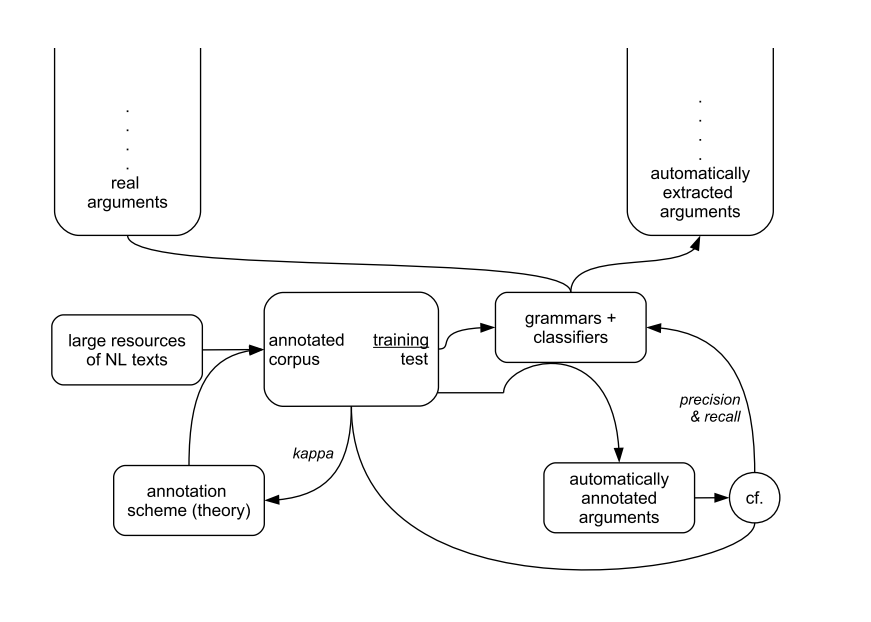
\includegraphics[scale=0.45]{images/NLP_techniques.png}
	\end{center}
	\caption{
		Natural language processing techniques
		\\
		\textbf{Source:} \cite{Budzynska2015}
	}
	\label{NLP_techniques}
\end{figure}

In general, argument mining procedure is separated into linguistic and computational part, as described in figure \ref{NLP_techniques}. Regarding the linguistic part, large corpora of manually annotated argument data are being created based on a common agreement among annotators about argument's structure. On the other hand, the computational part is separated into two main styles of automation, the structural and the statistical approach. (\cite{Budzynska2015}) \par

In \textbf{structural or grammar approach}, linguists aim to retrieve lexical patterns, rules or categories while annotating a training corpus. For example, it might be noticed that words like "because", "since", "however" are signs of arguments inside a specific corpus (\cite{Budzynska2015}). These signs are called indicators, and point out the connection between claims and premises inside a text (\cite{Lawrence2015}). Indicators are declared as linguistic expressions that connect statements and provide an unambiguous recognition of argumentative structure (\cite{Webber2012}). \par

A lot of research has been applied in order to be found words and expressions revealing argumentative structure (\cite{van2007argumentative}, \cite{knott1994using}). Apart from indicators, other structural techniques have been applied for argument mining. Such techniques are argumentation schemes (\cite{Feng2011}), dialogical context (\cite{Budzynska2014}), and semantic context (\cite{Cabrio2012}) or a combination of them. \par

In \textbf{statistical approach}, linguists are replaced by algorithms. These algorithms are basically classifiers developed for automating the argument annotation procedure (\cite{Budzynska2015}). The first attempts for the before mentioned automation were made in (\cite{Moens2007}), in which text is separated into sentences, and then each sentence is classified as argumentative or non-argumentative based on its lexical or syntactic features. As a result, (\cite{Palau2009}) presented an additional separation of argumentative sentences as premises or conclusions. As regards the automatic recognition of argumentative schemes, it was introduced in (\cite{Walton2011}) and it was based on the idea of connecting each scheme with a group of indicators. The paper's proposal is first indicating the arguments included in text, and then matching them to a given list of argument schemes. (\cite{Feng2011}) classifies annotated argumentation structures into a list of five common argumentation schemes. In (\cite{Lippi2015}), the authors describe a framework for claim detection in unstructured data-sets without any contextual information. Because arguments are often expressed through rhetorical structures, the previously mentioned framework was built based on an SVM classifier which captures similarities among parse trees via Tree Kernels. This method is used for measuring likeliness of two trees regarding their common substructures. Furthermore, Habernal and Gurevych (\cite{Habernalt2016}) try to evaluate argument convincingness by assessing their qualitative properties. Using an annotated corpus of 26,000 sentences, their purpose is to predict which argument is more convincing between a pair of arguments and to rank arguments regarding the topic and their convincingness, through the usage of SVM and LSTM algorithms. \par

Various traditional machine learning algorithms have been employed in the context of argument mining (Figure \ref{Machine_learning_algorithms}). More specifically, most of the  algorithms that have been implemented are Support Vector Machines (\cite{Mochales2011}; \cite{Park2015}; \cite{Stab2014}; \cite{Eckle-Kohler2015}), Logistic Regression (\cite{Levy2014}; \cite{Rinott2015}), Naive Bayes classifiers (\cite{Mochales2011}; \cite{Biran2011}; \cite{Park2015}; \cite{Eckle-Kohler2015}), Maximum Entropy classifiers (\cite{Mochales2011}), and Decision Trees and Random Forests (\cite{Stab2014}; \cite{Eckle-Kohler2015}). All mentioned classifiers are trained in labeled corpora. Thus, some parts of the annotated text are given, alongside with the associated label, and during training stage a model is being produced. This model is used to perform predictions on new unlabeled text. (\cite{Lippi2016}) \par

\begin{figure}[!h]
	\begin{center}
		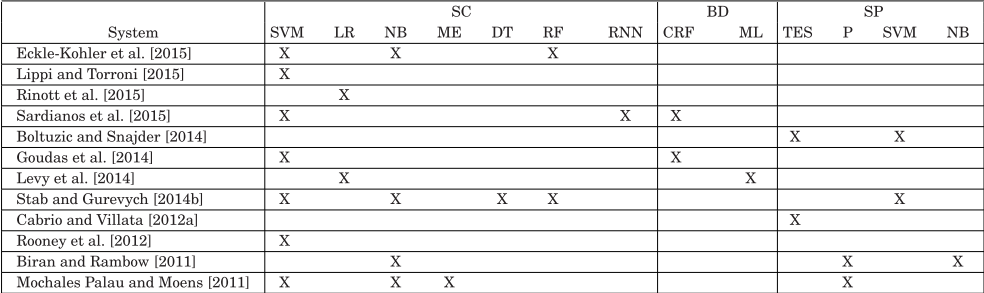
\includegraphics[scale=0.4]{images/Statistical-techniques_used.png}
	\end{center}
	\caption{
		Machine learning algorithms that have been used for argument mining
		\\
		\textbf{Source:} \cite{Lippi2016}
	}
	\label{Machine_learning_algorithms}
\end{figure}

Despite the fact that researchers have tried to make a comparison between these algorithms, there is no clear proof of which classifier is more appropriate for argumentation mining. In fact, most of the research efforts have been settled down on finding appropriate features for improving performance instead of implementing new specifically designed models and algorithms for solving argument identification problem (\cite{Lippi2016}). \par

To sum up, a number of different approaches have been applied to argument identification problem. The research community solutions are ranging from linguistic techniques (\cite{GarciaVillalba2012}) and topic modeling (\cite{Lawrence2014}), to supervised machine learning algorithms( firstly implemented by \cite{Moens2007}). \par

 
\chapter{Methods}

\label{Chapter3}

In this research paper, we attempt to apply two different approaches for recognizing argumentative sentences. These approaches cover both a structured methodology, which is related to the selection of hand-coded linguistic rules, and a statistical one, that includes the implementation of supervised algorithms; namely, Random Forest classifier and sequence classification with LSTM. \par

\section{Structural Approach}

The structural approach is based on lexical cues, rules or patterns for identifying arguments inside a given text. These cues are also referred to as argument indicators, since they are connecting claims and premises, signaling argumentative relations. \par


\addvbuffer[8pt 8pt]{
	\resizebox{0.92\linewidth}{!}{%
		\begin{tabular}{ |p{3.5cm}|p{1cm}|p{4cm}|p{3cm}|p{3.5cm}|p{1cm}|p{5cm}|p{2.5cm}| }
			\hline
			\multicolumn{8}{|c|}{ Argumentative Indicators based on (\cite{knott1994using})} \\
			\hline
			Indicator
								&POS
											&Indicator
																	&POS
					&Indicator
										&POS
													&Indicator
																						&POS\\
			\hline	
			even though			&none		&first					&adv
					&against			&none		&last								&adv\\
			naturally			&none		& most					&\{"[a-z]*ly": "adv"\}
					&if					&none		&(T|t)(he more).+?(the more)		&none\\
			once more			&none		&more					&\{"[a-z]*ly": "adv"\}
					&once again			&none		&(T|t)(he more).+?(the less)		&none\\
			surely				&none		&second					&adv
					&so					&mark		&third								&adv\\
			should say			&none		&too					&(too)(\$|[\textbackslash\textbackslash.])
					&might say			&none		&may say							&none\\
			could say			&none		&while					&mark
					&as a start			&none		&in order to						&none\\
			still				&adv		&that is				&none
					&since				&mark		&yet								&(Y|y)(et)[\^\textbackslash\textbackslash.].\\
			that				&mark		&above all				&none
					&actually			&none		&after all							&none\\
			afterwards			&none		&all in all				&none
					&also				&none		&although							&none\\
			anyway				&none		&as a consequence		&none
					&as a result		&none		&at any rate						&none\\
			at first blush		&none		&at first view			&none
					&at the outset		&none		&because							&none\\
			by comparison		&none		&by the same token		&none
					&certainly			&none		&consequently						&none\\
			correspondingly		&none		&despite the fact that	&none
					&either				&none		&equally							&none\\
			even then			&none		&every time				&none
					&except insofar as	&none		&firstly							&none\\
			for a start			&none		&for instance			&none
					&further			&none		&for the simple reason				&none\\
			accordingly			&none		&admittedly				&none
					&after that			&none		&all the same						&none\\
			alternatively		&none		&always assuming that	&none
					&as					&none		&as a corollary						&none\\
			at first			&none		&at first sight			&none
					&at the moment when	&none		&at the same time					&none\\
			but					&none		&by contrast			&none
					&by the way			&none		&clearly							&none\\
			conversely			&none		&despite that			&none
					&essentially		&none		&even so							&none\\
			eventually			&none		&except					&none
					&finally			&none		&first of all						&none\\
			for example			&none		&for one thing			&none
					&for this reason	&none		&furthermore						&none\\
			hence				&none		&in actual fact			&none
					&in any case		&none		&in conclusion						&none\\
			in fact				&none		&in other words			&none
					&in short			&none		&in sum								&none\\
			incidentally		&none		&instead				&none
					&merely because	 	&none		&just as							&none\\
			meanwhile			&none		&it might appear that	&none
					&as long as			&none		&as well							&none\\
			notably				&none		&moreover				&none
					&of course			&none		&nevertheless						&none\\
			on one hand			&none		&not only				&none
					&now that			&none		&no doubt							&none\\
			on the grounds that	&none		&on the assumption that	&none
					&on the one side	&none		&on the other side					&none\\
			plainly				&none		&otherwise				&none
					&so that			&none		&providing that						&none\\
			such that			&none		&secondly				&none
					&sure enough		&none		&simply because						&none\\
			thereafter			&none		&summing up				&none
					&therefore			&none		&suppose that						&none\\
			thirdly				&none		&the fact is that		&none
					&to be sure			&none		&though								&none\\
			to sum up			&none		&to conclude			&none
					&undoubtedly		&none		&to take an example					&none\\
			whenever			&none		&to the extent that		&none
					&whereas			&none		&what is more						&none\\
			wherever			&none		&for the reason that	&none
					&besides			&none		&(E|e)(ither).+?(or)				&none\\
			in one hand			&none		&(N|n)(either).+?(nor)	&none
					&on one side		&none		&in this case						&none\\
			in point of fact	&none		&as a matter of fact	&non
					&provided that		&none		&presumably							&none\\
			rather than			&none		&regardless				&none
					&as an example		&none		&simply								&none\\
			in order that		&none		& 						& 
					& 					& 			& 									& 	\\ 
					
			\hline
\end{tabular}}}

A list of indicators were extracted from the corpus created by (\cite{knott1994using}). This corpus includes often-used words or phrases in arguments according to paper's authors. Based on these words, a dictionary was developed containing as keys the extracted words, and as values, their specific part of speech in argumentative sentences. It needs to be mentioned that words, considered by us as usual or non-usual in argumentative structures, were added or removed respectively from the dictionary. For this purpose, there were created five methods in Python for paper's extraction, modification, as well as dictionary's creation (Appendix \ref{Appendix6}). The indicators that demonstrate the previously referred dictionary is presented in the table above. \par

Apart from dictionary's development, a way to handle and encapsulate corpora into the same format was necessary, and the code developed for this purpose is shown in Appendix \ref{Appendix7}. Each data-set was differently displayed, from unstructured text to sentence labeled data. This is the reason why there was created a \textit{datasets.ini} file containing information about data, for example the number of column indicating the sentence or/and the label, which sheet includes the desired data, or which is the data-set's path. The key of each record was the name of every corpora as it was saved in local file. So, depending on the data-set's type (excel, csv or txt file) and its configurations, other actions were applied in order to returned a list of sentences and their labels in case corpora was annotated. \par

By using the previously created dictionary and corpora handler, argument identification had to take place (Appendix \ref{Appendix8}). For this reason, part of speech tagging was necessary, so as a sentence's words and their POS to be compared to those words included in the dictionary. Statements tokenization was achieved through the usage of a library called \cite{spaCy}, which is an open-source NLP library written in Python and Cython, and it was selected due to its performance and efficiency comparing to other libraries. If any of matches between the dictionary and a given sentence occur, the sentence is characterized as argumentative, otherwise as non-argumentative. As regards the labeled corpora, the algorithm's outcomes and the given labels, which is considered to be the truth, are correlated so as four counters to be calculated; False Positives, False Negatives, True Positives and True Negatives. These counters are used for measuring accuracy that is a metric for reviewing algorithm's results, which will be used and described at Chapter \ref{Chapter5}. \par

\section{Statistical Approach}

The statistical approach is relying on algorithms developed for automating the argument annotation process. These algorithms receive as input, a representation of data that can be understood by computers. For this reason, textual data of our corpora need to be transformed into numeric tensors. (\cite{Chollet2017}) \par

Text is considered as a form of sequence data, and tokens are the different units into which a text can be split. These units can be either words, characters or n-grams (\cite{Chollet2017}). After text tokenization, the next step is connecting numeric vectors with the occurred tokens. Then, the sequences of vectors instead of words is fed into the selected algorithm. \par

There are a variety of ways for vector and token association. Two and the most known ones for forms of sequence data are the one-hot encodingText and word-embedding methods (\cite{Chollet2017}), which will be used in the implemented algorithms later on. 

As regards one-hot encodingText is a basic way to transform tokens into vectors. Every word is connected with a unique integer index, which is turned into a binary vector of vocabulary's size. Another version of this method is the one-hot hashing trick, which is used when vocabulary's unique tokens are too much that is difficult to be handled. This approach hashes words into a fixed-sized vector through a hashing function, rather than allocating an index to each word, and then creating a dictionary for these indexes. The disadvantages of this method is the hash collisions, and in general the inability of word's correlation that leads to high dimentionality. (\cite{Chollet2017})

Word embedding, or dense word vectors, is another popular way to associate vectors with words. In contrast with one-hot encodingText, this technique has low-dimensionality and float vectors. Furthermore, dense word vectors are trained by the data provided, and thus packing more and more data into the same dimensions. This is achieved by minimizing the geometric distance between related words, like synonyms, while maximizing it when words have different semantic (\cite{Chollet2017}).

The implemented algorithms for argument mining problem are the Random Forest classification algorithm, using one-hot encodingText, and the LSTM-RNN algorithm, using word embedding method. The annotation of argumentative and non-argumentative sentences can be considered as a binary classification in Random Forest (\cite{Stab2014}) or a statistical structure mapping of written language in LSTM (\cite{Chollet2017}).

\subsection{Random Forest Classification Algorithm}

The Random Forest algorithm is a collection of decision trees, where each one of them are slightly different from the others either by selecting the data-points or by selecting different features (\cite{Muller}). Every decision tree, built during the training period, predicts to which class a specific input is more suitable (argument or non-argument). After this process is completed, the chosen prediction for each sentence is the one that has the majority of votes across the decision trees. \cite{Chollet2017}

By using the \texttt{sklearn.ensemble} library, a Random Forest classification algorithm was implemented (Appendix \ref{Appendix9}). First of all, an annotated corpora containing both argumentative and non-argumentative sentences is loaded and features regarding how many words, punctuation characters and uppercase characters were created (see Chapter \ref{Chapter5}). Afterwords, the sentences were tokenized in order to be transformed into a format that computer can understand, as mentioned before. For the tokenization \texttt{OneHotEncoder} of \texttt{sklearn.preprocessing} library was used. The corpora was seperated into a training and a test set of data, and then model was defined and trained using the train data. Finally, the model is tested and a matrix showing the real and the predicted data was presented in a heatmap plot.

The model is applied by using two different methods for training. The one method is using the features created, like in (\cite{Lawrence2016}), while the other is by using the tokenized sentences.

\subsection{LSTM-RNN Algorithm}

Deep learning in natural-language processing problems is aiming to identify patterns of words or sentences (\cite{Chollet2017}). The most appropriate deep learning model for sequence data processing, like sequences of words in our case, is the Recurrent Neural Network algorithm. RNN is a neural network algorithm that is implementing internal iterations. The RNN resets its state every time a new independent process occurs, which means that each sequence is a different data input to the network. However, network include loops over each sequence's elements. RNN includes the so-called LSTM layer. The Long Short-Term Memory algorithm was developed by Hochreiter and Schmidhuber in 1997, and the purpose of creation was to solve the "vanishing-gradient problem" of SimpleRNN algorithm. LSTM is basically allowing previous information to be re-injected across different timesteps. (\cite{Chollet2017})

By using the tensorFlow keras API, an LSTM algorithm was conducted and implemented (Appendix \ref{Appendix10}). First of all, the corpora created in Chapter \ref{Appendix4} is loaded, and data applied to one list of sentences and one list of labels. Following, the corpora is split into a training and a testing data-set. Furthermore, the lists of trained sentences were tokenized, taking into account only the first ten-thousand most frequent words. The lists of the occurred trained sequences, which are basically lists of integers after the tokenization process, are transformed into a two-dimensions numpy array that has a shape of (number of sequences, number of timesteps). The number of timesteps is basically the length of the longest sequence. It has to be mentioned that shorter sequences are padded with values at the end, so every sequence has the same shape.

As regards word embedding, Global Vectors for Word Representation (\cite{glove}) was used, which is a file containing 100-dimensional pre-computed embedding vectors for 400,000 of English words. This file helped in building an index that associates words with number vectors, and through which an embedding matrix of shape (max\_words= 10000, embedding\_dim = 100) was created and loaded in Embedding layer later on. The Embedding layer is a dictionary-like that maps integer indexes for certain words to dense vectors, and it is the first layer of our model. The second layer applies to LSTM method, while the third layer of Dense was added to end our stack of layers with an equal number of units and classes created. After constructing our model, we are freezing the Embedding layer to avoid deleting what has already been learned. 

Finally, the model was trained based on the training data, which are explicitly separated into training and validation samples used for learning word embedding based on our corpora. The last step is testing the model on the test data by firstly tokenizing the sentences, and then evaluating the results occurred.

\chapter{Data Curation}

\label{Chapter4} 
In order to successfully apply the statistical learning approach, a well-structured training data-set is needed. In this section, the process of data curation is elaborated so as both argumentative and non-argumentative sentences to be found. \par

Most of the argumentative sentences included in our corpora were found on two IBM data-sets created for this purpose (Table \ref{argData}), and are about three main topics; Video Games, Democracy and Multiculturalism. It has to be mentioned that some of the data were duplicated, and thus Python code of Appendix \ref{Appendix2} was created so as to be removed. \par

\begin{table}[H]
	\centering
	\resizebox{0.8\linewidth}{!}{%
		\begin{tabular}{ |p{2.2cm}|p{4cm}|p{2cm}|p{2cm}|p{2cm}|p{2cm}| }
			\hline
					Source Data 
							&file
																&Total Data
																		&Duplicated
																				&Arguments  
																						&Non-Arguments\\
			\hline
			\cite{aharoni2014benchmark} 
							&CDEdata.xls						&1292   &967	&325	&-  \\
			\cite{bar-haim-etal-2017-stance}	
							&claim\_stance\_dataset\_v1			&2394  	&56		&2366	&-  \\ % ??
			
			\hline
		\end{tabular}
	}
	\caption{Argumentative Data Used} 
	\label{argData}
\end{table}

However, the exploitation of the existing annotated data-sets regarding argument detection has the obstacle of lacking non-argumentative instances. The previously mentioned IBM corpora contain only phrases that have been manually annotated as positive instances of arguments. This means that it is impossible to train a supervised algorithm in classifying non-arguments without any negative examples. \par

So, our purpose was to gather an equal number of argumentative and non-argumentative sentences that have the same context with the curated data of IBM. Therefore, plain text referring to Video Games was found in additional IBM data-sets. These raw data files were split into sentences, and each of these sentences was labeled as argument or non-argument by authors of this research paper, and the Table \ref{argNonArgData} depicts the results. The data referred as "Not used" were blank or incomplete lines. \par

The non-arguments collected were not enough, thus it was decided to scrap data from Wikipedia articles. The topics of these articles were similar to the previously gathered data, and more specifically about Video games, Democracy and Multiculturalism. The code used for the scraping process, as weel as the scraped pages, are aligned at Appendix \ref{Appendix1}. \par

\begin{table}[H]
	\centering
	\resizebox{0.75\linewidth}{!}{%
		\begin{tabular}{ |p{2cm}|p{4cm}|p{2cm}|p{2cm}|p{2cm}|p{2cm}| }
			\hline
			Source Data 
			&file
																&Total Data
																		&Not Used
																				&Arguments  
																						&Non-Arguments\\
		\hline
		\cite{mirkin2017recorded}   
			&asr/DJ\_1\_ban-video-games\_pro.wav.asr.txt		&9	 	&3		&5		&1  \\
		\cite{mirkin2017recorded}   
			&asr/EH\_1\_ban-video-games\_pro.wav.asr.txt		&20 	&3		&12		&5  \\ 
		\cite{mirkin2017recorded}   
			&asr/HE\_1\_ban-video-games\_pro.wav.asr.txt		&21 	&1		&12		&8  \\ 
		\cite{mirkin2017recorded}   
			&asr/SN\_1\_video-games\_pro.wav.asr.txt			&28 	&10		&15		&3  \\
		\cite{mirkin2017recorded}   
			&asr/TL\_1\_ban-video-games\_pro.wav.asr.txt		&19 	&6		&8		&5  \\
		\cite{mirkin2017recorded}   
			&asr/YB\_1\_ban-video-games\_pro.wav.asr.txt		&19 	&4		&7		&8  \\ 
		\cite{aharoni2014benchmark} 
			&wiki12\_articles/Gender
			\_representation\_in\_video\_games					&39  	&4		&5		&30  \\
																				%2755	%60
		\hline
	\end{tabular}}
	\caption{Argumentative and Non-Argumentative Data Used} 
	\label{argNonArgData}
\end{table}

Assuming that Wikipedia articles' authors are objective and do not express their point of view, most of the data scraped were included as non-arguments in the data-set. It has to be mentioned that the data collected from this procedure were previously checked from the python code-described in the Chapter \ref{Chapter3} ( Appendix \ref{Appendix6}). The sentences classified as non-arguments were added to the created data-set, while the others were considered as ambiguous (Table \ref{nonArgContrData}).\par


\begin{table}[H]
	\centering
	\resizebox{0.75\linewidth}{!}{%
		\begin{tabular}{ |p{8.7cm}||p{2.5cm}|p{2.6cm}|p{2.7cm}|p{2.8cm}|}
			\hline
				Topic of Wikipedia
																	&Total Data
																			&Not Used
																					&Controversial sentences 
																							&Non-Arguments\\
		\hline
		Early Hstory of video games									&143	&19		&59		&65		\\
		Fourth generation of video game consoles					&65		&6		&32		&27 	\\
		Game Boy													&84		&22		&23		&39		\\
		Game design													&223	&32		&71		&120	\\
		Game														&191	&28		&89		&74		\\
		Gaming Computer	`											&129	&8		&62		&59		\\
		Gaming disorder												&12		&6		&-		&6		\\
		History of video games										&604	&70	    &224    &310	\\
		Home computer												&359	&236	&54		&69		\\
		Nintendo													&393	&70		&133	&190	\\
		PC game														&248	&60	    &87	    &101	\\
		Video game													&434	&82		&154	&198	\\
		Video game addiction in China								&58		&4		&9		&45		\\
		Video game addiction										&257	&138	&70		&49		\\
		Video game console											&337	&261	&41		&35		\\
		Video game culture											&292	&74		&104	&114 	\\
		Video game development										&446	&229	&102	&115 	\\
		Video game industry											&275	&49		&91		&135	\\
		Video game music											&460	&176	&146	&138	\\
		Video game programmer										&164	&19		&72		&82		\\
		Video game-related health problems 							&52		&7		&22		&23		\\
		Video gaming in Japan										&300	&102	&82		&116	\\
		Video gaming in the United States							&119	&31		&27		&61		\\
		The Game Awards												&36		&2		&18		&16		\\
		Multicultural transruption					 				&45		&3		&20		&22		\\
		Multicultural and diversity management 						&41		&7		&17		&17		\\
		Multicultural education										&248	&28		&104	&116	\\
		Multiculturalism in Australia								&156	&37		&55		&54		\\
		Criticism of multiculturalis								&237	&56		&96		&85		\\
		Cultural pluralism											&28		&7		&12		&9		\\
		Multiculturalism in Canada									&205	&28		&84		&93		\\
		Multiculturalism											&449	&62		&160	&227	\\
		Democracy Index												&59		&18		&17		&24		\\
		Direct democracy											&162	&22		&59		&81		\\
		Types of democracy											&25		&7		&9		&9		\\
		Representative democracy									&56		&7		&26		&23		\\
		Criticism of democracy										&191	&102	&55		&34		\\
		Athenian democracy											&335	&41		&147	&147	\\
		History of democracy										&394	&81		&126	&187	\\
		Democracy													&452	&71		&193	&188	\\
																					%2952	%3503
	    \hline
	\end{tabular}}
	\caption{Non-Argumentative Data Used \& Controversial Sentences} 
	\label{nonArgContrData}
\end{table}

The previously described data were concatenated (Appendix \ref{Appendix3}), so as to be used in the statistical approach algorithms. The corpora is composed by both arguments and non-arguments (Table \ref{nonArgContrData}). \par 

\begin{table}[H]
	\centering
	\resizebox{0.75\linewidth}{!}{%
		\begin{tabular}{ |p{3cm}|p{2cm}|p{2cm}|p{2cm}|p{2.8cm}| }
			\hline
			\multicolumn{5}{|c|}{Argumentative and No-Argumentative Data Used} \\
			\hline
			File				&Total Data		&Arguments  &Non-Arguments &False-Positive Arguments\\
			\hline
			
			dataset.csv			&6318			&2755		&3563		   &-	\\
			found\_fp.csv		&2952			&-			&-			   &2952 \\
	    \hline
	\end{tabular}}
	\caption{Data included in our corpora} 
	\label{argNonArgDataUsed}
\end{table}

As regards the ambiguous sentences of Wikipedia articles that was mentioned before, they were all saved in a file named \texttt{found\_ambiguous.csv} (Appendix \ref{Appendix4}). This file indicates all the keywords responsible for these controversial results. The indicators- described in the previous Chapter and found in Wikipedia articles- were counted using code of Appendix \ref{Appendix5}, and the following table was the outcome of that enumeration. \par
	
\begin{table}[H]
	\centering
	\resizebox{.55\linewidth}{!}{%
		\begin{tabular}{ |p{4cm}|p{1cm}|p{5cm}|p{1cm}| }
			\hline
				Indicator Found
									&Number of Sentences
													&Indicator Found
																				&Number of Sentences \\
				\hline
				\textbf{as}			&\textbf{968}	&\textbf{that}				&\textbf{542}	\\
				\textbf{also}		&\textbf{440}	&\textbf{because}			&\textbf{121}	\\
				\textbf{as well}	&\textbf{101}	&\textbf{for example}		&\textbf{92}	\\
				(E|e)(ither).+?(or)	&44	 			&as a result				&23 			\\
				\textbf{because}	&\textbf{121}	&notably					&13				\\
				for instance		&17				&\textbf{but}				&\textbf{326}	\\
				that is				&40				&\textbf{while}				&\textbf{197}	\\
				actually			&26				&against					&3				\\
				still				&85				&so that					&12				\\
				though				&87				&besides					&4				\\
				furthermore			&13				&eventually					&41				\\
				\textbf{more +}		&\textbf{40}	&either						&53				\\
				clearly				&5				&\textbf{if}				&\textbf{107}	\\
				since				&34				&on the grounds that		&3				\\
				although			&85				&third						&6 				\\
				consequently		&4				&as a consequence			&2				\\
				rather than			&66				&instead					&42				\\
				nevertheless		&9 				&except						&5				\\
				otherwise			&12				&in fact					&10				\\
				too					&3				&not only					&22				\\
				on one side			&1				&simply						&26 			\\
				moreover			&9				&hence						&4				\\
				therefore			&25				&every time					&1				\\
				in other words		&4				&despite the fact that		&2				\\
				in order to			&43				&as							&9				\\
				at the same time	&7				&of course					&2				\\
				finally				&13				&as an example				&2				\\
				first				&29				&even though				&14				\\
				lastly				&3				&equally					&7				\\
				whereas				&13				&(T|t)(he more).+?(the more)&2				\\
				regardless			&7				&for this reason			&2				\\
				simply because		&1				&by contrast				&3				\\
				naturally			&4				&at any rate				&1				\\
				in short			&2				&in this case				&3				\\
				such that			&5				&essentially				&5				\\
				(N|n)(either).+?(nor)&4				&whenever					&4				\\
				second				&5				&as long as					&2				\\
				even then			&3				&as a matter of fact		&1				\\
				accordingly			&3				&provided that				&1				\\
				conversely			&3				&alternatively				&3				\\
				afterwards			&6				&thereafter					&1				\\
				meanwhile			&10				&once again					&3				\\
				once more			&1				&above all					&1				\\
				by comparison		&1				&surely						&2 				\\
				undoubtedly			&2				&on the one side			&1				\\
				at first			&1				&presumably					&2				\\
				after all			&1				&what is more				&1				\\
				certainly			&1				&anyway						&1				\\
				so					&16				&most						&22				\\
				\textbf{further}	&\textbf{53}	&							&				\\
	   		\hline
			\end{tabular}}
	\caption{Indicators found in Wikipedia articles} 
	\label{indicators}
\end{table}

The goal of this process was to test in Wikipedia articles the argumentative indicators included in the Chapter \ref{Chapter3}'s dictionary, and upon cross-examination to remove indicators that do not usually reveal argumentative sentences. Based on the Table \ref{indicators}, the indicators marked as bold are the ones found in the majority of Wikipedia sentences. More than 10\% of each indicator's sentences was examined by the authors of this research papers, and the keywords, that did not usually pointed out argumentative statements and removed from the dictionary, are represented in the following. The annotations are described in detail inside the file \texttt{Results/found\_ambiguous\_results\_annotated.xlsx}.

\begin{table}[H]
	\centering
	\resizebox{.9\linewidth}{!}{%
		\begin{tabular}{ |p{4cm}|p{3cm}|p{3cm}|p{3cm}|p{3cm}|p{3cm}|p{3cm}| }
			\hline
				Indicator
										&Total Number of Sentences
												&Number of Sentences Examined
													&Arguments
														&Non-Argument
															&Depending on the context
																&Removed from the dictionary\\
			\hline

				as						&968	&131&22	&98	&11	&Yes 	\\
				that					&542	&91	&20	&54	&17	&Yes 	\\
				also					&440	&64	&8	&46	&10	&Yes 	\\
				but						&326	&50	&7	&36	&7	&Yes 	\\
				while					&197	&35	&6	&24	&5	&Yes 	\\
				because					&121	&33	&20	&10	&3	&No		\\
				if						&107	&20	&6	&12	&2	&No		\\
				as well					&101	&20	&5	&14	&1	&No		\\
				for example				&92		&8	&5	&3	&0	&No		\\
				further					&53		&20	&4	&15	&1	&Yes	\\
				against					&51		&21	&3	&16	&2	&Yes	\\
				more +a dverb in 'ly'	&40		&16	&4	&12	&0	&No		\\
				
			\hline
		\end{tabular}}
	\caption{Indicators found in Wikipedia articles} 
	\label{removed_indicators}
\end{table}

It was also observed that the following indicators were used in combination with punctuation, and that's why they were modified into the formats of the table \ref{modified_indicators}.

\begin{table}[H]
	\centering
	\resizebox{.4\linewidth}{!}{%
		\begin{tabular}{ |p{4cm}|p{3cm}|p{3cm}|p{3cm}|p{3cm}|p{3cm}|p{3cm}| }
			\hline
			Indicator
									&Modified to\\
			\hline
			
			while					&, while 		\\
			that is					&, that is, 	\\
			still					&, still	 	\\
			as a result				&as a result,	\\
			
			\hline
	\end{tabular}}
	\caption{Indicators found in Wikipedia articles} 
	\label{modified_indicators}
\end{table}



\chapter{Results}

\label{Chapter5}

Results for both structured and statistical implementations presented in Chapter \ref{Chapter3}, are applied to a set of corpora in order to be evaluated. \par

\section{Structural Approach}

The structural approach described in previous chapters is being assessed into this section. For this purpose, the code of Appendix \ref{Appendix8} alongside with two IBM corpora was applied. It has to be mentioned that these two IBM corpora include only argumentative sentences, and we aim to check how many of those arguments will be identified correctly by our algorithm. 

The metric of accuracy was used in order to evaluate the indicators selected for recognizing argumentative sentences, while precision, recall and f1 score did not have value because of the non-arguments lack. For measuring accuracy, four counters were used; \textbf{true positives} (tp) is counting the times both algorithm and analyst labeled a sentence as argumentative, \textbf{true negatives} (tn) how often both algorithm and analyst labeled as non-argumentative, \textbf{false positive} (fp) the times the algorithm assigned as argumentative a sentence that expert recognized as non-argumentative, \textbf{false negative} (fn) how many times human identified a sentence as argumentative while algorithm did not. 

\begin{itemize}
 	\item \textbf{Accuracy} represents the percentage of correctly classified sentences:
 	\[ A
 	= \dfrac{tp + tn}{tp + tn + fp + fn}
 	\]
 	\item \textbf{Precision} indicates the times of correctly identification instances:
 	\[ P
 	= \dfrac{tp}{tp + fp}
 	\]
 	\item \textbf{Recall} measures the times algorithm missed out arguments:
 	\[ R
 	= \dfrac{tp}{tp + fn}
 	\]
 	\item \textbf{F1 Score} presents the mean of precision and recall:
 	\[ F
 	= \dfrac{2*P*R}{P + R}
 	\]
\end{itemize} 

\begin{table}[H]
	\centering
	\resizebox{0.65\linewidth}{!}{%
	\begin{tabular}{ | p{2cm} |  p{4cm} | p{2cm} | }
		\hline
		\textbf{Source Data} 
				& \textbf{file} 			
						& \textbf{Accuracy}  		\\[0.5cm] \hline
										
		\cite{bar-haim-etal-2017-stance}
				&claim\_stance\_dataset\_v1
						&17.50\%					\\[0.2cm] 
		\cite{Aharoni2014}
				&CDEdata.xls1.00.1480.25
						&14.81\%					\\[0.2cm]
		\hline
	\end{tabular}}
	\caption{Results of Structural Approach} 
	\label{structural_approach_results}
\end{table}

Structural approach seems not to be able to capture a variety of argumentative structures. This is beacause, argumentative patterns are rarely used in practice, since human discourse involves a lot of information which is being implied rather than being explicitly stated.

\newpage
\section{Statistical Approach}

\subsection{Random Forest Algorithm}
Supervised machine learning algorithms need a number of labeled data in order to be trained. That was the reason corpora of Chapter \ref{Chapter4} was created, and used in the implantation of Random Forest classifier algorithm (Appendix \ref{Appendix9}). A number of 33\% of the data used to train the model, while the rest of them to evaluate the results. 

It has to be mentioned that two methods were used for argument's classification. The first one was by tokenizing the sentences, so as to be in a format that a computer can understand, and then training the model based on the tokenized sentences. This method had an accuracy of \textbf{56.83\%}, precision \textbf{100\%}, recall \textbf{0.55\%}, f1 score \textbf{71.13\%}, and the results are displayed in the heatmap of figure \ref{random_forest} (A). Based on the results, it seems that Random Forest trained by tokenized sentencses is not recognizing argumentative sentences. That's why we implemented another technique in which we determined some features of each sentence ,and then feed the algorithm with these features instead of the sentences. In this way the accuracy increased to \textbf{79.42\%}, while precision is \textbf{74.08\%}, recall \textbf{78.72\%}, f1 score \textbf{76.33\%} , and it deprecates to the heatmap of figure \ref{random_forest} (B). The results of the first approach are not that high, and that is probably because of the unique words.

The features used for classification are the following based on the paper (\cite{Lawrence2016}):

\begin{itemize}
	\item \textbf{Word Counter}: the number of words in a sentence
	\item \textbf{Uppercase Characters Counter}: the number of uppercase characters found
	\item \textbf{Punctuation or Special Characters Counter}: the number of presence punctuation characters like " "
\end{itemize} 

\begin{figure}[H]
	\centering
	\subfloat[Classification based 
	on the sentences]{{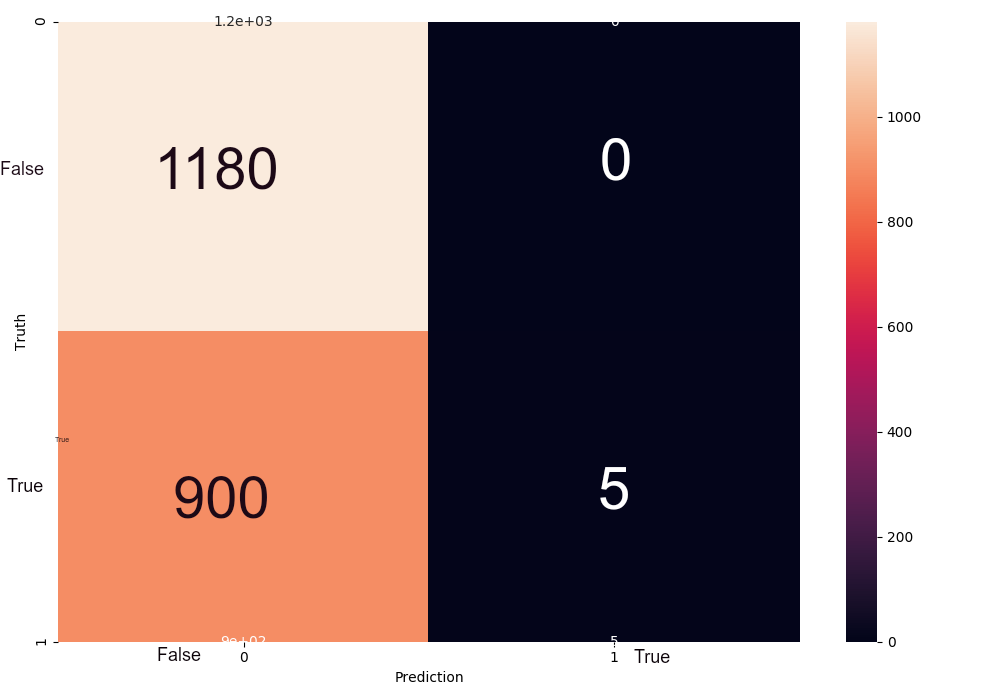
\includegraphics[scale=0.2]{images/random_forest_sentences.png} }}%
	\qquad
	\subfloat[Classification based 
	on features]{{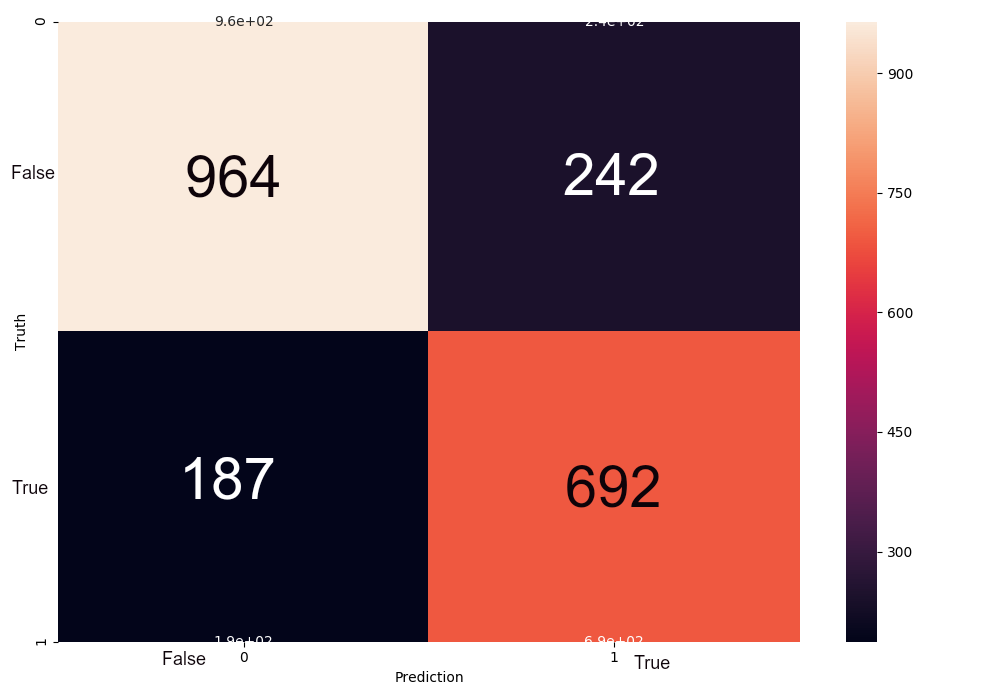
\includegraphics[scale=0.2]{images/random_forest_features.png} }}%
	\caption{
		Predicted and Real results of Random Forest classification algorithm
	}
	\label{random_forest}
\end{figure}

As the results of table \ref{random_forest} reveal, Random Forest implements well when features are used for each of sentence. Machine learning approach seems to be a better fit for identifying arguments than lexical rules.

\subsection{LSTM-RNN Algorithm}

The LSTM-RNN algorithm described in previous chapters is being assessed into this section. For this purpose, the code of Appendix \ref{Appendix10} alongside with the data-set described in Chapter \ref{Chapter4} was executed.

The data-set used contains an equal number of argumentative and non-argumentative sentences, as well as their labels. The twenty percent of the data were used for training the model, while the rest of them for evaluating it. The model's performance over time is represented in the following plots by using the metrics of accuracy and loss. 

\begin{figure}[H]
	\centering
	\subfloat[]{{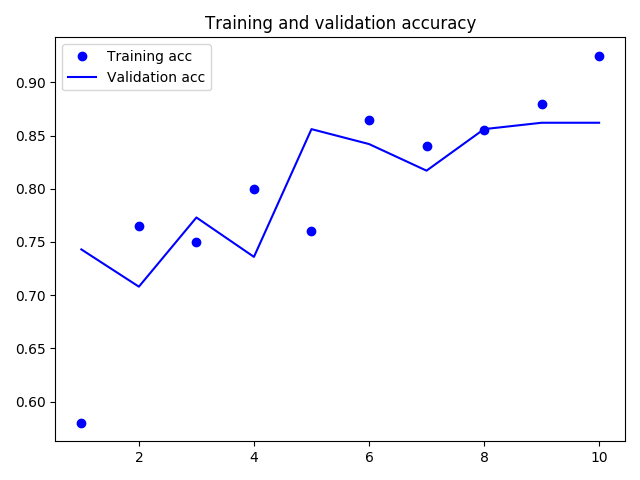
\includegraphics[scale=0.31]{images/machine_learning_accuracy.png} }}%
	\qquad
	\subfloat[]{{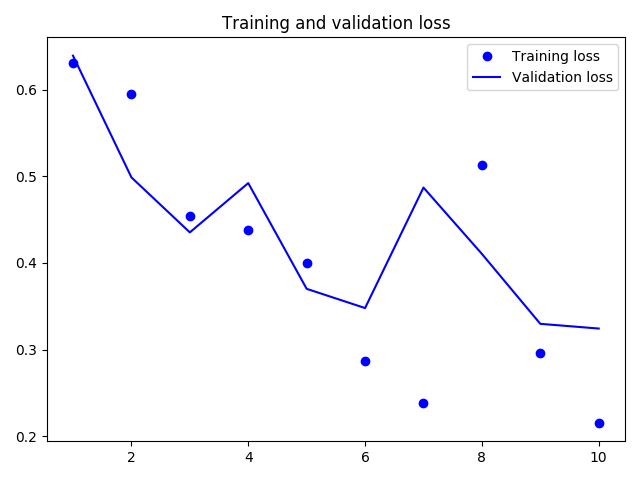
\includegraphics[scale=0.31]{images/machine_learning_acc.png} }}%
	\caption{
		Training and validation accuracy and loss when using pretrained word embeddings
	}
	\label{fig:example}
\end{figure}

After testing the algorithm in test data, the following results occurred with an accuracy of \textbf{85.36\%}, precision \textbf{78.15\%}, recall \textbf{88.90\%}, f1 score \textbf{82.61\%}. These results lead to a conclusion that LSTM-RNN algorithm seems to be more appropriate for argument mining problems, comparing to Random Forest and the Structural approach examined in the previous section.

\begin{lstlisting}[language=bash]
Found 10823 unique tokens.
Shape of data tensor: (5054, 235)
Shape of label tensor: (5054,)
Found 400000 word vectors.

Model: "sequential"
_________________________________________________________________
Layer (type)                 Output Shape              Param #   
=================================================================
embedding (Embedding)        (None, None, 100)         1000000   
_________________________________________________________________
lstm (LSTM)                  (None, 100)               80400     
_________________________________________________________________
dense (Dense)                (None, 1)                 101       
=================================================================
Total params: 1,080,501
Trainable params: 1,080,501
Non-trainable params: 0
_________________________________________________________________
None

Train on 200 samples, validate on 1000 samples
Epoch 1/10
200/200 [==============================] - 2s 10ms/sample - loss: 0.6307 - acc: 0.6350 - f1_m: 0.3386 - precision_m: 0.9722 - recall_m: 0.2519 - val_loss: 0.6393 - val_acc: 0.6090 - val_f1_m: 0.6948 - val_precision_m: 0.5351 - val_recall_m: 0.9980
Epoch 2/10
200/200 [==============================] - 2s 9ms/sample - loss: 0.5955 - acc: 0.6250 - f1_m: 0.4697 - precision_m: 0.7757 - recall_m: 0.5645 - val_loss: 0.4988 - val_acc: 0.8390 - val_f1_m: 0.8320 - val_precision_m: 0.7773 - val_recall_m: 0.8969
Epoch 3/10
200/200 [==============================] - 1s 7ms/sample - loss: 0.4542 - acc: 0.8700 - f1_m: 0.8178 - precision_m: 0.8778 - recall_m: 0.7895 - val_loss: 0.4353 - val_acc: 0.8150 - val_f1_m: 0.8213 - val_precision_m: 0.7220 - val_recall_m: 0.9551
Epoch 4/10
200/200 [==============================] - 1s 7ms/sample - loss: 0.4383 - acc: 0.8000 - f1_m: 0.7469 - precision_m: 0.8571 - recall_m: 0.7411 - val_loss: 0.4922 - val_acc: 0.7600 - val_f1_m: 0.7883 - val_precision_m: 0.6582 - val_recall_m: 0.9867
Epoch 5/10
200/200 [==============================] - 1s 7ms/sample - loss: 0.3999 - acc: 0.8250 - f1_m: 0.8295 - precision_m: 0.8415 - recall_m: 0.8676 - val_loss: 0.3702 - val_acc: 0.8500 - val_f1_m: 0.8494 - val_precision_m: 0.7830 - val_recall_m: 0.9289
Epoch 6/10
200/200 [==============================] - 1s 6ms/sample - loss: 0.2866 - acc: 0.9050 - f1_m: 0.8928 - precision_m: 0.8759 - recall_m: 0.9155 - val_loss: 0.3480 - val_acc: 0.8490 - val_f1_m: 0.8474 - val_precision_m: 0.7793 - val_recall_m: 0.9292
Epoch 7/10
200/200 [==============================] - 1s 7ms/sample - loss: 0.2383 - acc: 0.9050 - f1_m: 0.9028 - precision_m: 0.8486 - recall_m: 0.9646 - val_loss: 0.4870 - val_acc: 0.7960 - val_f1_m: 0.7277 - val_precision_m: 0.9137 - val_recall_m: 0.6066
Epoch 8/10
200/200 [==============================] - 1s 6ms/sample - loss: 0.5132 - acc: 0.7800 - f1_m: 0.7525 - precision_m: 0.7843 - recall_m: 0.8197 - val_loss: 0.4105 - val_acc: 0.8100 - val_f1_m: 0.7571 - val_precision_m: 0.8881 - val_recall_m: 0.6615
Epoch 9/10
200/200 [==============================] - 1s 6ms/sample - loss: 0.2962 - acc: 0.8850 - f1_m: 0.8746 - precision_m: 0.9322 - recall_m: 0.8448 - val_loss: 0.3297 - val_acc: 0.8650 - val_f1_m: 0.8500 - val_precision_m: 0.8417 - val_recall_m: 0.8593
Epoch 10/10
200/200 [==============================] - 1s 6ms/sample - loss: 0.2154 - acc: 0.9500 - f1_m: 0.9505 - precision_m: 0.9344 - recall_m: 0.9677 - val_loss: 0.3243 - val_acc: 0.8710 - val_f1_m: 0.8628 - val_precision_m: 0.8376 - val_recall_m: 0.8928
1264/1264 [==============================] - 1s 938us/sample - loss: 0.3474 - acc: 0.8536 - f1_m: 0.8261 - precision_m: 0.7815 - recall_m: 0.8890
Accuracy: 85.36%
Precision: 78.15%
Recall: 88.90%
F1 score: 82.61%
\end{lstlisting}

 
% Chapter Template

\chapter{Conclusion}
\label{Chapter6}

I have implemented three separate argument mining techniques, applicable to both structural and statistical approach. For the \textbf{structural approach}, there was created a dictionary of lexical cues that usually characterize argumentative structures based on (\cite{knott1994using}). The algorithm created was tested in two IBM corpora containing only argumentative sentences, the accuracy seems to be around \textbf{15 to 17 \%}. As regards the statistical approach, a corpora has to be curated in order to include both argumentative and non-argumentative instances. That is why Wikipedia articles were scrapped assuming that there are no arguments included, and the sentences gathered were cross-checked by the algorithm created for the structural approach. Every sentence that did not have argumentative cues, based on the algorithm, was added to the corpora as non-argumentative, while the others considered as ambiguous and were checked by two annotators so as to remove misleading indicators of dictionary. Afterwards, two algorithms were built by using as training data a part of this corpora. \textbf{Random forest classification algorithm} was approached by two different methods of training. The first technique was by using the tokenized sentences which leads to an accuracy of \textbf{56.83\%}, precision \textbf{100\%}, recall \textbf{0.55\%}, f1 score \textbf{71.13\%}, while the second was by using features like counter of words, uppercase and punctuation characters that have an accuracy of \textbf{79.42\%},  precision \textbf{74.08\%}, recall \textbf{78.72\%}, and f1 score \textbf{76.33\%}. Finally, the other algorithm of statistical approach that was built is the \textbf{LSTM-RNN} that concludes to an accuracy of \textbf{85.44\%}, precision of \textbf{78.15\%}, recall of \textbf{88.90\%}, f1 score of \textbf{82.61\%}. 

As the results of both structural and statistical algorithms reveal, linguistic rules are not capable of successfully identifying arguments. On the other hand, learning algorithms are a better fit to argument mining, with the most accurate one to be the LSTM-RNN algorithm. One of the main goals as regarding future work is to apply the algorithms built in a fully annotated data-set found in GitHub's issues. 

%----------------------------------------------------------------------------------------
%	REFERENCES
%----------------------------------------------------------------------------------------

\printbibliography[title={References}]

%----------------------------------------------------------------------------------------
%	Appendicies
%----------------------------------------------------------------------------------------

\addcontentsline{toc}{part}{Appendicies}
\setcounter{chapter}{1}
\addtocontents{toc}{\protect\setcounter{tocdepth}{0}}%

\disableboldchapterintoc
\part*{Appendicies}

%\removechapterspaces
\renewcommand\chaptername{Appendicies}
\setcounter{chapter}{0}

% Appendix 1

\chapter{Scrap Data from Wikipedia}

\label{Appendix1}

\begin{lstlisting}[language=iPython]
import urllib.request
import re
from inscriptis import get_text


def wiki(theme):
	url = "https://en.wikipedia.org/wiki/" + theme
	html = urllib.request.urlopen(url).read().decode('utf-8')
	
	text = get_text(html)
	
	with open('../datasets/wiki_' + theme + '.txt', 'w') as out:
		for row in text.split('\n'):
			if len(row) >= 80 and not row[0].isdigit() and not row[1].isdigit() and not row[2] == '*':
				row = re.sub(r'\[\d+]', '', row)
				row = row.rstrip('\n')
				out.write(row)
				out.write('\n')


if __name__ == '__main__':
	
	# Video games topic
	wiki('Video_game-related_health_problems')
	wiki('Video_game_addiction_in_China')
	wiki('Video_game_addiction')
	wiki('Gaming_disorder')
	wiki('2017_in_video_gaming')
	wiki('2019_in_video_gaming')
	wiki('History_of_video_games')
	wiki('PC_game')
	wiki('Video_game_culture')
	wiki('Gaming_computer')
	wiki('Video_game_console')
	wiki('Video_game')
	wiki('Video_gaming_in_the_United_States')
	wiki('Video_game_music')
	wiki('Video_game_industry')
	wiki('Video_game_development')
	wiki('Game_design')
	wiki('Video_game_programmer')
	wiki('Early_history_of_video_games')
	wiki('Video_gaming_in_Japan')
	wiki('Video_game_crash_of_1983')
	wiki('Sixth_generation_of_video_game_consoles')
	wiki('Video_gaming_in_China')
	wiki('1980s_in_video_gaming')
	wiki('Home_computer')
	wiki('Nintendo')
	wiki('Game_Boy')
	wiki('Fourth_generation_of_video_game_consoles')
	wiki('Game')
	wiki('The_Game_Awards')
	
	# Democracy topic
	wiki('Democracy')
	wiki('History_of_democracy')
	wiki('Athenian_democracy')
	wiki('Representative democracy')
	wiki('Direct_democracy')
	wiki('Types_of_democracy')
	wiki('Democracy_Index')
	wiki('Criticism_of_democracy')
	
	# Multiculturalism
	wiki('Multiculturalism')
	wiki('Criticism_of_multiculturalism')
	wiki('Cultural_pluralism')
	wiki('Multiculturalism_in_Canada')
	wiki('Multicultural_education')
	wiki('Multicultural_and_diversity_management')
	wiki('Multiculturalism_in_Australia')
	wiki('Multicultural_transruption')
	
\end{lstlisting}

% Appendix 2

\chapter{Remove Duplicate Sentences}

\label{Appendix2}

\begin{lstlisting}[language=iPython]
import os

FILE_PATH = os.path.abspath(os.path.dirname(__file__))


def remove_duplicate_rows(file_name):
	sentences = []
	
	with open(os.path.join(FILE_PATH, '../Results/' + file_name), mode='r') as txt_file:
		reader = txt_file.read()
		
		for sentence in reader.split("\n"):
			sentences.append(sentence)
	
	with open ( os.path.join ( FILE_PATH, '../Results/new_' + file_name ), mode='w' ) as txt_file_new:
		for i in range(len(sentences)):
			if i == 0:
				txt_file_new.write(sentences[i])
				txt_file_new.write("\n")
			elif i < len(sentences) and sentences[i] != sentences[i-1]:
				txt_file_new.write(sentences[i])
				txt_file_new.write("\n")


if __name__ == '__main__':
	remove_duplicate_rows('CDEdata.csv')
	
\end{lstlisting}

% Appendix 3

\chapter{Concat Results of checked Data}

\label{Appendix3}

\begin{lstlisting}[language=iPython]
import os
import glob
import csv

FILE_PATH = os.path.abspath(os.path.dirname(__file__))


def combine_results():

	csvfiles = glob.glob(FILE_PATH + '/../Results/checked/*.csv')
	dataset = csv.writer(open(FILE_PATH + '/../Results/dataset.csv', 'w'), delimiter=',')
	
	for files in csvfiles:
		rd = csv.reader(open(files, 'r'))
		
		for row in rd:
			if 'wiki' in files:
				if "False" in row:
					dataset.writerow(row)
			else:
				if "True" or "False" in row:
					dataset.writerow(row)


def find_ambiguous():

	csvfiles = glob.glob(FILE_PATH + '/../Results/checked/*.csv')
	found_ambiguous = csv.writer(open(FILE_PATH + '/../Results/found_ambiguous.csv', 'w'), delimiter=',')
	
	for files in csvfiles:
		rd = csv.reader(open(files, 'r'))
		
		for row in rd:
			if 'wiki' in files:
				if "True" in row:
					found_ambiguous.writerow(row)
		

if __name__ == '__main__':
	combine_results()
	find_ambiguous()

\end{lstlisting}
% Appendix 4

\chapter{Gather Ambiguous Sentences found in Wiki articles}

\label{Appendix4}

\section{../Results/found\_ambiguous\_results.csv}

In the \textbf{terminal} type: 
\begin{lstlisting}[language=bash]
	$python3 getAmbiguousSentences.py > ../Results/found_ambiguous_results.csv
\end{lstlisting}

\section{getAmbiguousSentences.py}
%TO DO remove dublicated code and add the diff code in another file, check the code if it is properly executed

\begin{lstlisting}[language=iPython]
import json
from configParser import choose_function
from getArguments import spaCy, pos_tagged, check_regex

"""
Description: by using a dictionary that includes words often used 
in arguments, it is identified if given sentences are 
arguments or not. Part of speech tagging from spaCy is used 
for this purpose as well and it is imported by getArguments.py file.
"""


def check_dictionary(doc, dictionary):
	"""None
	This function checks if any of the words in the sentence exists
	 in the dictionary given. If it does, then it is checked if 
	 this word's part of speech match with its value given in 
	 dictionary. If they match, then the word is added in a 
	 list named keyword_found.
	
	:param doc: pos tagged sentence from spacy function
	:param dictionary: dictionary that has as keywords words 
		and as value their part of speech
	:return: keywords found in the given sentence
	"""
	
	keyword_found = []
	
	for key, value in dictionary.items():
		if check_regex(doc, key) is not None:
			if len(value) == 1:
				for key2 in value:
					if checz_regex(doc, key + ' ' + key2) is not None 
					 and check_regex(doc, key2) is not None and 
					 pos_tagged(doc, check_regex(doc, key2).text) is not 'None':
						if value[key2] == pos_tagged(doc, check_regex(doc, key2).text)[1] or \
						 value[key2] == pos_tagged(doc, check_regex(doc, key2).text)[2]:
							keyword_found.append(key + " + " + key2)
			elif value == 'none':
				keyword_found.append(key)
			elif len(value) != 1 and check_regex(doc, value) 
			 is not None:
				keyword_found.append(key)
			elif pos_tagged(doc, key)[1] == value or \
			 pos_tagged(doc, key)[2] == value:
				keyword_found.append(key)
	
	return keyword_found


if __name__ == '__main__':

	with open('../dict/dictionary.json', 'r') as dict:
		dictionary = json.load(dict)
	
	sentences = choose_function("found_ambiguous.csv")
	
	if sentences != 'No dataset found':
		for sentence in sentences:
		
			print('"' + str(sentence[0]).strip('b') + '",' + 
				str(check_dictionary(spaCy(sentence[0]), dictionary))
		
	else:
		print(sentences)
\end{lstlisting}

% Appendix 5

\chapter{Enumerate ambiguous sentences}

\label{Appendix5}

\begin{lstlisting}[language=iPython]
import os
import csv
import json

FILE_PATH = os.path.abspath(os.path.dirname(__file__))


def enumerate_ambiguous(file_name):
	with open('../dict/dictionary.json', 'r') as dict:
		dictionary = json.load(dict)
	
		with open(os.path.join(FILE_PATH, '../Results/' + file_name), mode='r', encoding='utf-8') as file:
			reader = csv.reader(file)
			counters = {}
			
			count = 0
			count_rows = 0
			
			for row in reader:
				firstArgumentWordFlag = False
				
				count_rows += 1
				# first cell includes sentences, not keywords
				for column in row[1:]:
				
					if firstArgumentWordFlag == False:
						testStr = "['"
							if column.startswith(testStr):
							firstArgumentWordFlag = True
						else:
							continue
					
					column = column.strip("['] ")
					column = column.strip('"')
					
					if column in dictionary:
						count += 1
						if column in counters:
							counters[column] += 1
						else:
							counters[column] = 1
					else:
						if ' + ' in column:
							count += 1
							firstPart = column.split(" + ")[0]
							
							if firstPart in counters:
								counters[firstPart] += 1
							else:
								counters[firstPart] = 0
						else:
							print(row)
							print('Not found: ', column)

	save_array_to_csv(counters)


def save_array_to_csv(my_dict):
	with open(FILE_PATH + '/../Results/found_Ambiguous_keywords.csv', 'w', newline='') as f:
		w = csv.writer(f)
		w.writerows(my_dict.items())


if __name__ == '__main__':
	enumerate_ambiguous('found_ambiguous_results.csv')

\end{lstlisting}

% Appendix 6

\chapter{Extract keywords from pdf}

\label{Appendix6}

\begin{lstlisting}[language=iPython]
"""
Description: extract words which are often used in arguments 
(based on a paper),and create a dictionary based on these words
(key of the dict) and their specific, if they have one, part
of speech (value of the dict) in arguments
"""

import json
import textract
import os
import csv

FILE_PATH = os.path.abspath(os.path.dirname(__file__))  # path of this file


def extract_data():
	"""
	By using textract library, this function extracts the whole pdf file
	
	pdf: paper called 'Using Linguistic Phenomena to Motivate a Set
	of Coherence Relations'
	"""
	
	text = textract.process(os.path.join(FILE_PATH,
	"../Reading/cues-UsingLinguisticPhenomenaMotivateCoherenceRelations_Knott93.pdf"))
	save(text)


def save(text):
	"""
	This function saves extracted text to a csv file
	"""
	if not os.path.exists("../dict" ):
		os.makedirs("../dict")
		
	with open(os.path.join(FILE_PATH, "../dict/data.csv"),
	 mode='wb') as csv_file:
		csv_file.write(text)
		
	modify_csv_file("../dict/data.csv")  # modify extracted text


def modify_csv_file(data):
	"""
	This function modifies csv file in order to keep those words 
	we are interested in
	"""
	
	flag = 0
	
	with open(os.path.join(FILE_PATH, data)) as inp:
		reader = csv.reader(inp)
		
		with open(os.path.join(FILE_PATH, "../dict/data2.csv"),
		 mode='w') as out:
			for row in reader:
				if len(row) > 0 and row[0] == "Phrase":
					flag = 1
					continue
				if len(row) == 0 or row[0].isdigit():
					flag = 0
				if flag == 1 and len(row) > 0:
					out.write(row[0])
					out.write("\n")
	check_words("../dict/data2.csv", "../dict/data.csv")


def check_words(data2, data):
	"""
	This function adds or removes words that considered as useful 
	or not
	"""
	
	exclude_words = ['after', 'and', 'as soon as', 'before', 
					'at first',	'at first sight', 'earlier', 
					'fisrt of all',	'for', 'inasmuch as', 
					'later', 'much sooner', 'not because',
					'now', 'if not', 'if so', 
					'in the beginning', 'in the end', 
					'in the meantime', 'in turn', 
					'much later', 'not', 'notwithstanding that', 
					'suppose', 'the more often', 'this time', 
					'presumably because', 'when', 'where',
					'previously', 'regardless of that', 'rather', 
					'after that', 'as',	'simply because', 'then', 
					'true', 'until', 'again', 'and/or', 'or', 
					'else', 'even']
	
	include_words = ['for the reason that', 'besides', 
					'(E|e)(ither).+?(or)','(N|n)(either).+?(nor)', 
					'in one hand', 'in this case',	'on one side',
					'as a matter of fact', 'in point of fact',	
					'presumably', 'provided that', 
					'regardless', 'rather than', 'simply', 
					'as an example', 'in addition']
	
	test_words = {'even though': 'none', 'first': 'adv', 
				'against': 'none', 'last': 'adv',
				'more': {'[a-z]*ly': 'adv'}, 
				'most': {'[a-z]*ly': 'adv'}, 'if': 'none',
				'(T|t)(he more).+?(the more)': 'none', 
				'(T|t)(he more).+?(the less)': 'none', 
				'naturally': 'none', 'once again': 'none', 
				'once more': 'none', 'surely': 'none',
				'second': 'adv', 'so': 'mark', 'third': 'adv', 
				'too': '(too)($|[\.])', 'should say': 'none',
				'might say': 'none', 'may say': 'none', 
				'could say': 'none', 'while': 'mark', 
				'as a start': 'none', 'in order to': 'none',
				'in order that': 'none', 'still': 'adv', 
				'that is': 'none', 'since': 'mark', 
				'yet': '(Y|y)(et)[^\.].', 'that': 'mark'}
	
	with open(os.path.join(FILE_PATH, data2), 'r') as inp, \
		open(os.path.join(FILE_PATH, data), 'w') as out:
		
		for row in csv.reader(inp):
			if row[0] in exclude_words:
				continue
			else:
				out.write(row[0])
				out.write("\n")
		
		for word in include_words:
			out.write(word)
			out.write("\n")
	
	create_dictionary("../dict/data.csv", test_words)


def create_dictionary(data, test_words):
	"""
	This function creates a .json file that includes a dictionary of 
	the	words from the csv file created before and some additional 
	words for testing
	"""
	
	dictionary = test_words
	
	with open(os.path.join(FILE_PATH, data), 'r') as inp:
	
		for row in csv.reader(inp):
			if "\x05" in row[0]:
				row[0] = row[0].replace('\x05', 'fi')  # correct words from pdf extraction
			
			if row[0] in test_words.keys():
				continue
			else:
				dictionary.update({row[0]: 'none'})

	with open('../dict/dictionary.json', 'w') as dict:
		json.dump(dictionary, dict)


if __name__ == '__main__':
	extract_data()

\end{lstlisting}

% Appendix 7

\chapter{Load Data-sets based on their configurations}

\label{Appendix7}

\begin{lstlisting}[language=iPython]
from xlrd import open_workbook
import configparser
import os
import re
import csv

FILE_PATH = os.path.abspath(os.path.dirname(__file__))


def py23_str(value):
	"""
	This function tries to convert a string to unicode. Because 
	of the fact that this conversion differ from python 3
	to python 2, here are checked both possibilities so as 
	the program to run in both python 3 and 2.
	
	:param value: sentence to be converted from string to unicode
	:return: converted input
	"""
	
	try:  # Python 2
		return unicode(value, errors='ignore', encoding='utf-8')
	except NameError:  # Python 3
		try:
			return str(value, errors='ignore', encoding='utf-8')
		except TypeError:  # Wasn't a bytes object, no need to decode
			return str(value)


def get_sentences_csv(dataset_number):
	"""
	This function reads files with .csv extension
	
	:dataset_number: number that refers to order (starts from 0) 
	of a dataset in datasets.ini
	
	:return: a list of sentences
	"""
	sentences = []
	
	path, _, column, is_argument = get_parameters_dataset(dataset_number)
	
	with open(os.path.join(FILE_PATH, path), mode='r') as dataset:
		reader = csv.reader(dataset)
		for sentence in reader:
			if is_argument is not None:
				sentences.append([str(sentence[int(column)]), str(sentence[int(is_argument)])])
			else:
				sentences.append([str(sentence[int(column)]), 'True'])
	
	sentences.pop(0)
	return sentences


def get_sentences_xls(dataset_number):
	"""
	This function reads files with .xls extension
	
	:dataset_number: number that refers to order (starts from 0) 
	of a dataset in datasets.ini
	:return: a list of sentences
	"""
	sentences = []
	
	path, sheet, column, is_argument = get_parameters_dataset(dataset_number)
	
	reader = open_workbook(path, on_demand=True)
	sheet = reader.sheet_by_name(sheet)
	if is_argument is not None:
		for cell, cell2 in zip(sheet.col(int(column)), sheet.col(int(is_argument))):
			sentences.append([cell.value.encode("utf-8"), cell2.value.encode("utf-8")])
	else:
		for cell in sheet.col(int(column)):
			sentences.append([cell.value.encode("utf-8"), 'True'])
	
	sentences.pop(0)
	return sentences


def get_sentences_txt(dataset_number):
	"""
	This function reads files with .txt or none extension
	
	:dataset_number: number that refers to order (starts from 0) 
					 of a dataset in datasets.ini
	
	:return: a list of sentences
	"""
	sentences = []
	
	path, _,  _, _ = get_parameters_dataset(dataset_number)
	
	with open(os.path.join(FILE_PATH, path), mode='r') as txt_file:
		reader = txt_file.read()
		
		for sentence in reader.split('.'):
			sentences.append([sentence])
	
	return sentences


def get_parameters_dataset(dataset):
	"""
	This function gets the arguments of a specific dataset from datasets.ini
	
	:dataset: number that refers to order (starts from 0) 
			  of a dataset or the name of dataset in datasets.ini
	:return: section['path'] + file_name: path of dataset
	sheet: sheet that data are in it if it is an .xls file
	column: column of sentences to be identified as arguments or not
	is_argument: column which reveals if a specific sentence is 
				 an argument or not
	"""
	dataset_number, config = check_validity_of_dataset(dataset)
	
	section = config.sections()[dataset_number]  # each section is a name of a file with data
	section = config[section]
	file_name = re.match(r".*: (.*)>", str(section), re.MULTILINE)
	file_name = file_name.group(1)
	
	try:
		sheet = section['sheet']
	except KeyError:
		sheet = None
	
	try:
		is_argument = section['is_argument']
	except KeyError:
		is_argument = None
	
	try:
		column = section['column']
	except KeyError:
		column = None
	
	return section['path'] + file_name, sheet, column, is_argument


def check_validity_of_dataset(dataset):
	"""
	This function checks of a dataset exists in dataset.ini or not
	
	:dataset: number that refers to order (starts from 0) of 
	a dataset or the name of dataset in datasets.ini
	:return: dataset_number: returns the order of given 
	dataset in datasets.ini	config: returns object config 
	from datasets.ini
	"""
	config = configparser.ConfigParser()
	config.read('../datasets/datasets.ini')
	
	if dataset in config:
		dataset_number = config.sections().index(dataset)
	elif dataset < len(config.sections()):
		dataset_number = dataset
	
	return dataset_number, config


def choose_function(dataset):
	"""
	This function checks the extension of a datasets and chooses 
	an appropriate method to read the file
	
	:dataset: number that refers to order (starts from 0) 
	of a dataset or the name of dataset in datasets.ini
	:return: a list of sentences if dataset exits 
	otherwise 'No dataset found'
	"""
	
	try:
		dataset_number = int(check_validity_of_dataset(dataset)[0])
		
		try:
			_, extension = dataset.rsplit('.', 1)
		except ValueError:
			extension = None
			
		if extension == 'xls':
			return get_sentences_xls(dataset_number)
		elif extension == 'csv':
			return get_sentences_csv(dataset_number)
		elif extension == 'txt' or extension is None:
			return get_sentences_txt(dataset_number)
		
	except TypeError:
		return 'No dataset found'

\end{lstlisting}

% Appendix 8

\chapter{Find Argumentative Sentences}

\label{Appendix8}

\begin{lstlisting}[language=iPython]
import json
import spacy
from __future__ import division
from configParser import choose_function, os, py23_str, re

"""
Description: by using a dictionary that includes words often used 
in arguments, this file identifies if given sentences are 
arguments or not. Part of speech tagging from spaCy is used 
for this purpose as well.
"""

FILE_PATH = os.path.abspath(os.path.dirname(__file__))

tp = 0
tn = 0
fp = 0
fn = 0


def spaCy(sentence):
	"""
	By using spaCy, this function gets a sentence and returns every
	word's part of speech
	
	:param sentence: input to be tokenized
	:return: tokenized sentence
	"""
	
	nlp = spacy.load('en')
	doc = nlp(py23_str(sentence))
	
	return doc


def pos_tagged(doc, word):
	"""
	This function gets a tagged sentence from spaCy and a specific 
	word and return its part of speech and its dependency
	
	:param doc: pos tagged sentence from spacy function
	:param word: a word that we are interested to learn its part of 
		speech
	:return: word, its part of speech(pos) and its dependence in the
		given sentence or None
	"""
	
	word = word.lower()
	
	for token in doc:
		if token.text.lower() == word:
			return [token.text, token.pos_.lower(), token.dep_.lower()]
	
	return 'None'


def check_regex(doc_regex, regex):
	"""
	By using spaCy's function called match, this function is
	checking if a specific regular expression is represented
	by a given sentence
	
	:param doc_regex: pos tagged sentence from spacy function
	:param regex: a regular expression
	:return: the part of the sentence that is indicated in the given
		regex otherwise None
	"""
	
	regex = re.compile(r''+regex)
	
	for match in re.finditer(regex, doc_regex.text.lower()):
		start, end = match.span()  # get matched indices
		word_found = doc_regex.char_span(start, end)  # create Span from indices
		
		return word_found
	
	return None


def check_dictionary(doc, dictionary):
	"""
	This function checks if any of the words in the sentence exists
	 in the dictionary given. If it does, then it is checked if 
	 this word's part of speech match with its value given in 
	 dictionary. If they match, then the word is added in a 
	 list named keyword_found.
	
	:param doc: pos tagged sentence from spacy function
	:param dictionary: dictionary that has as keywords words 
		and as value their part of speech
	:return: True if the list keyword_found is not empty or False 
			 if it is empty
	"""
	
	keyword_found = []
	
	for key, value in dictionary.items():
		if check_regex(doc, key) is not None:
			if len(value) == 1:
				for key2 in value:
					if checz_regex(doc, key + ' ' + key2) is not None 
					 and check_regex(doc, key2) is not None and 
					 pos_tagged(doc, check_regex(doc, key2).text) is not 'None':
						if value[key2] == pos_tagged(doc, check_regex(doc, key2).text)[1] or \
						 value[key2] == pos_tagged(doc, check_regex(doc, key2).text)[2]:
							keyword_found.append(key + " + " + key2)
			elif value == 'none':
				keyword_found.append(key)
			elif len(value) != 1 and check_regex(doc, value) 
			 is not None:
				keyword_found.append(key)
			elif pos_tagged(doc, key)[1] == value or \
			 pos_tagged(doc, key)[2] == value:
				keyword_found.append(key)
	
	if len(keyword_found) != 0:
		return 'True'
	else:
		return 'False'


def check_validity(real_value, given_value):
	"""
	This function checks if two given values match
	
	:param real_value:  real value is the result of check_dictionary
		function
	:param given_value: given value is the value given by analysts 
		into dataset
	:return: Correct results if they match or Wrong results if they
		do not match
	"""
	global tn, tp, fn, fp
	
	if real_value in given_value:
		if real_value == 'True':
			tp = tp + 1
		else:
			tn = tn + 1
		return "Correct results"
	else:
		if real_value == 'False':
			fp = fp + 1
		else:
			fn = fn + 1
		return "Wrong results"


def precision():
	if (tp + fp) != 0:
		return tp/(tp + fp)
	else:
		return "Integer division by zero"


def recall():
	if (tp + fn) != 0:
		return tp/(tp + fn)
	else:
		return "Integer division by zero"


def f1_score(precision, recall):
	if (precision + recall) != 0:
		return 2 * (precision * recall) / (precision + recall)
	else:
		return "Integer division by zero"


if __name__ == '__main__':

	with open('../dict/dictionary.json', 'r') as dict:
		dictionary = json.load(dict)
	
	sentences = choose_function("found_fp.csv")
	labeled_data = False
	
	if sentences != 'No dataset found':
        for sentence in sentences:

			if len(sentence) == 2:
				print('"' + str(sentence[0]).strip('b') + '",' + 'True') # for csv
				# print ( str ( sentence[0] ).strip ( 'b' ) + ',' + 'True' )
				labeled_data = True
				
			else:
				print('"' + str(sentence[0]).strip('b') + '",' + 
				 check_dictionary(spaCy(sentence[0]), dictionary)) # for csv
	
	else:
		print(sentences)
\end{lstlisting}

% Appendix 9

\chapter{Statistical Approach: Random Forest algorithm}

\label{Appendix9}

\begin{lstlisting}[language=iPython]
import pandas as pd
import seaborn as sn
from sklearn.preprocessing import OneHotEncoder
from sklearn.model_selection import train_test_split
from sklearn.ensemble import RandomForestClassifier
from sklearn.metrics import confusion_matrix
import matplotlib.pyplot as plt
import string
import csv
import os
import numpy as np


"""
Description: implementing Random Forest classifier model
to an annotated corpora that contains 
both argumentative and none sentences
"""

FILE_PATH = os.path.abspath(os.path.dirname(__file__))  # path of this file


def load_dataset(path):
	"""
	Loading dataset of a given path, and creating features based on the sentences given.
	The first feature is a counter of words included in each sentence,
	the second feature is a counter of uppercase characters, while
	the third feature is a counter of special characters (punction)
	:param path: full path of dataset
	:return: a list of sentences and their labels, and a set of features
	"""
	
	# load & prepare data
	with open(path, 'r') as file:
		dataset = csv.reader(file, delimiter=",")
		df = pd.DataFrame(dataset)
	
	del df[2]  # column full of non	labels = df[1]
	df[1] = [len(sentences.split()) for sentences in df[0]]  # Word Count'
	df[2] = [sum(char.isupper() for char in sentence) \
			for sentence in df[0]]  # 'Uppercase Char Count'
	
	df[3] = [sum(char in string.punctuation for char in sentence) \
			for sentence in df[0]]  # 'Special Char Count'
	df[4] = pd.factorize(labels)[0]  # switch False to 0 and True to 1
	
	return df


def tokenize_sentences(df):
	"""
	Tokenizing raw sentences by using One-hot encoding
	into a format that a computer can understand
	
	:param df: the dataframe that includes 4 columns
				[sentences, word Counter, uppercase counter,
				special char counter, label]
	:return: tokenized sentences, labels
	"""
	vectorizer = OneHotEncoder(handle_unknown='ignore')
	vectorizer.fit([[line.strip()] for line in df[0]])
	sentences = vectorizer.transform([[line.strip()] for line in df[0]]).toarray()
	
	# sentences = vectorizer.fit_transform(df[0])
	labels = df[4]
	return sentences, labels


def define_model(x_train, y_train):
	"""
	This function defines and trains the Random Forest model
	
	:param x_train: the training sentences
	:param y_train: the sentences' labels
	:return: trained model
	"""
	model = RandomForestClassifier()
	model.fit(x_train, y_train)
	return model


def testing_model(model, x_test, y_test):
	"""
	This function evaluates the model on the test set
	
	:param model: trained model
	:param x_test: the testing set of sentences
	:param y_test: the sentences' labels
	:return: a matrix of the predicted and real values
	"""
	score = model.score(x_test, y_test)
	print("Accuracy: %.2f%%" % (score * 100))
	
	y_predicted = model.predict(x_test)
	cm = confusion_matrix(y_test, y_predicted)
	print(cm)
	return cm


def plot_results(cm):
	"""
	This function is showing a heatmap plot based on
	the values of the confusion matrix that contains
	the real an predicted values.
	:param cm: matrix of both real and predicted values
	"""
	plt.figure(figsize=(10, 7))
	sn.heatmap(cm, annot=True)
	plt.xlabel('Prediction')
	plt.ylabel('Truth')
	plt.show()


if __name__ == '__main__':
	df = load_dataset('../Results/dataset.csv')
	sentences, labels = tokenize_sentences(df)
	
	#  using features instead of the sentences
	#
	features = np.asarray(df[df.columns[1:4]].values)
	# split dataset into test and train data
	x_train, x_test, y_train, y_test = \
		train_test_split(features, labels, test_size=0.33)
	
	model = define_model(x_train, y_train)
	cm = testing_model(model, x_test, y_test)
	plot_results(cm)
	
	#  using sentences without their features
	#
	# split dataset into test and train data
	x_train, x_test, y_train, y_test = train_test_split(sentences, labels, test_size=0.33)
	
	model = define_model(x_train, y_train)
	cm = testing_model(model, x_test, y_test)
	plot_results(cm)

\end{lstlisting}

% Appendix 10

\chapter{Statistical Approach: LSTM-RNN algorithm}

\label{Appendix10}

\begin{lstlisting}[language=iPython]
import csv
import os
import pandas as pd
import numpy as np
import matplotlib.pyplot as plt
from sklearn.model_selection import train_test_split
from tensorflow.python.keras.preprocessing.text import Tokenizer
from tensorflow.python.keras.preprocessing.sequence \
	import pad_sequences
from tensorflow.python.keras.layers import Dense, LSTM, Embedding
from tensorflow.python.keras.models import Sequential
from keras import backend

"""
Description: implement lstm model to an annotated corpora
that contains both argumentative and none sentences
"""

# path of this file
FILE_PATH = os.path.abspath(os.path.dirname(__file__))


def load_dataset(path):
	"""
	Loading dataset of a given path
	:param path: full path of dataset
	:return: a list of sentences and their labels
	"""
	
	# load & prepare data
	with open(path, 'r') as file:
		dataset = csv.reader(file, delimiter=",")
		df = pd.DataFrame(dataset)
	
	del df[2]  # column full of none
	
	df[1] = pd.factorize(df[1])[0]  # False switched to 0 and True to 1
	texts = list(df[0].values)
	labels = list(df[1])
	
	return texts, labels


def get_tokenized_text(max_words, texts_train):
	"""
	Tokenizing raw sentences.
	:param max_words: considering only the top max_words of dataset 
					  (most frequent ones)
	:param texts_train: sentences to for tokenization
	:return: tokenizer, sequences, word_index
	"""
	tokenizer = Tokenizer(num_words=max_words)
	tokenizer.fit_on_texts(texts_train)
	sequences = tokenizer.texts_to_sequences(texts_train)
	word_index = tokenizer.word_index
	
	print('Found %s unique tokens.' % len(word_index))
	return tokenizer, sequences, word_index


def pad_sentences(sequences, labels_train):
	"""
	This function transforms a list of num_sentences sequences
	(lists of integers) into a 2D Numpy array of shape 
	(num_sentnece, num_timesteps).
	The num_timesteps is either the maxlen argument if provided,
	or the length of the longest sequence otherwise.
	Sequences that are shorter than num_timesteps are padded 
	with value at the end.
	
	:param sequences: list of tokenized sentences
	:param labels_train: list of sequences' labels
	:return: a 2D Numpy array of sentences and labels
	"""
	data = pad_sequences(sequences)
	labels_train = np.asarray(labels_train)
	print('Shape of data tensor:', data.shape)
	print('Shape of label tensor:', labels_train.shape)
	
	# Splits the data into a training set and a validation set, 
	# but first shuffles the data
	indices = np.arange(data.shape[0])
	np.random.shuffle(indices)
	data = data[indices]
	labels_train = labels_train[indices]
	
	return data, labels_train


def word_embedding(glove_file, max_words, word_index):
	"""
	Parsing the GloVe's word-embeddings file in order 
	to build an index that maps words (as strings) 
	to their vector representation (as number vectors),
	and then build an embedding matrix that will 
	be loaded into an Embedding layer later on.
	
	:param glove_file: path of Glove's word-embedding
	:param max_words: considering only the top max_words 
					  of dataset (most frequent ones)
	:param word_index: index of words after tokenization
	:return: embedding_dim, embedding_matrix 
			 of shape (max_words, embedding_dim)
	"""
	
	embeddings_index = {}
	f = open(os.path.join(FILE_PATH, glove_file))
	for line in f:
		values = line.split()
		word = values[0]
		coefs = np.asarray(values[1:], dtype='float32')
		embeddings_index[word] = coefs
	f.close()
	print('Found %s word vectors.' % len(embeddings_index))
	
	embedding_dim = 100
	embedding_matrix = np.zeros((max_words, embedding_dim))
	for word, i in word_index.items():
		if i < max_words:
			embedding_vector = embeddings_index.get(word)
			if embedding_vector is not None:
				# Words not found in the embedding 
				# index will be all zeros.
				embedding_matrix[i] = embedding_vector
	
	return embedding_dim, embedding_matrix


def lstm_model(max_words, embedding_dim, embedding_matrix):
	"""
	This function defines the model and
	loads pretrained word embedding into the Embedding layer
	
	:param max_words: considering only the top max_words 
					  of dataset (most frequent ones)
	:param embedding_dim: number of embedding dimensions used
	:param embedding_matrix: a matrix of shape shape 
							 (max_words, embedding_dim)
	:return: the defined model
	"""
	
	# define model
	model = Sequential()
	model.add(Embedding(max_words, embedding_dim))
	model.add(LSTM(100))
	model.add(Dense(1, activation='sigmoid'))
	print(model.summary())
	
	# Loading pretrained word embeddings into the Embedding layer
	model.layers[0].set_weights([embedding_matrix])
	model.layers[0].trainable = False
	
	return model
	
	
def recall_m(y_true, y_pred):
	"""
	Calculating recall metric
	
	:param y_true: the real value of a sentence
	:param y_pred: the estimated value of a sentence
	:return: recall metric
	"""
	true_positives = backend.sum(backend.round(backend.clip(y_true * y_pred, 0, 1)))
	possible_positives = backend.sum(backend.round(backend.clip(y_true, 0, 1)))
	recall = true_positives / (possible_positives + backend.epsilon())
	return recall


def precision_m(y_true, y_pred):
	"""
	Calculating precision metric
	
	:param y_true: the real value of a sentence
	:param y_pred: the estimated value of a sentence
	:return: precision metric
	"""
	true_positives = backend.sum(backend.round(backend.clip(y_true * y_pred, 0, 1)))
	predicted_positives = backend.sum(backend.round(backend.clip(y_pred, 0, 1)))
	precision = true_positives / (predicted_positives + backend.epsilon())
	return precision


def f1_m(y_true, y_pred):
	"""
	Calculating F1 Score metric
	
	:param y_true: the real value of a sentence
	:param y_pred: the estimated value of a sentence
	:return: f1_score metric
	"""
	precision = precision_m(y_true, y_pred)
	recall = recall_m(y_true, y_pred)
	return 2 * ((precision * recall) / (precision + recall + backend.epsilon()))


def training_model(x_train, y_train, x_val, y_val, model):
	"""
	This function is responsible for compiling and
	training the model
	
	:param x_train: sentences for training model (200 sentences)
	:param y_train: labels of training sentences
	:param x_val: sentences for validating trained model 
				  (1000 sentences)
	:param y_val: labels of validation sentences
	:param model: defined model
	:return: historing of training, trained model
	"""
	
	model.compile(loss='binary_crossentropy', optimizer='rmsprop',
				  metrics=['accuracy'])
	history = model.fit(x_train, y_train, epochs=10, batch_size=128,
						validation_data=(x_val, y_val))
	model.save_weights('pre_trained_glove_model.h5')
	
	return history, model


def plotting_results(history):
	"""
	This function is showing plots of the training and 
	validation results based on accuracy and loss metrics.
	
	:param history: history of training procedure
	"""
	acc = history.history['acc']
	val_acc = history.history['val_acc']
	loss = history.history['loss']
	val_loss = history.history['val_loss']
	epochs = range(1, len(acc) + 1)
	
	plt.plot(epochs, acc, 'bo', label='Training acc')
	plt.plot(epochs, val_acc, 'b', label='Validation acc')
	plt.title('Training and validation accuracy')
	plt.legend()
	plt.figure()
	
	plt.plot(epochs, loss, 'bo', label='Training loss')
	plt.plot(epochs, val_loss, 'b', label='Validation loss')
	plt.title('Training and validation loss')
	plt.legend()
	plt.show()


def testing_model(texts_test, labels_test, tokenizer, model):
	"""
	This function tokenizes the data of test set,
	and evaluates the model on the test set
	
	:param texts_test: sentences for testing model
	:param labels_test: labels of the testing sentences
	:param tokenizer: tokenizer
	:param model: trained model
	:return: accuracy of the created model
	"""
	
	# Tokenizing the data of the test set
	sequences = tokenizer.texts_to_sequences(texts_test)
	x_test = pad_sequences(sequences)
	y_test = np.asarray(labels_test)
	
	# Evaluating the model on the test set
	model.load_weights('pre_trained_glove_model.h5')
	loss, accuracy, f1_score, precision, recall = model.evaluate(x_test, y_test)
	
	print("Accuracy: %.2f%%" % (accuracy * 100))
	print("Precision: %.2f%%" % (precision * 100))
	print("Recall: %.2f%%" % (recall * 100))
	print("F1 score: %.2f%%" % (f1_score * 100))


def main():
	texts, labels = load_dataset('../Results/dataset.csv')
	texts_train, texts_test, labels_train, labels_test = \
		train_test_split(texts, labels, test_size=0.2)
	
	max_words = 10000  # Considers only the top 10,000 words 
					   # in the dataset
	training_samples = 200
	validation_samples = 1000\usepackage{xcolor}
	\definecolor{maroon}{cmyk}{0, 0.87, 0.68, 0.32}
	\definecolor{halfgray}{gray}{0.55}
	\definecolor{ipython_frame}{RGB}{207, 207, 207}
	\definecolor{ipython_bg}{RGB}{247, 247, 247}
	\definecolor{ipython_red}{RGB}{186, 33, 33}
	\definecolor{ipython_green}{RGB}{0, 128, 0}
	\definecolor{ipython_cyan}{RGB}{64, 128, 128}
	\definecolor{ipython_purple}{RGB}{170, 34, 255}
	
	tokenizer, sequences, word_index = \
		get_tokenized_text(max_words, texts_train)
	data, labels_train = pad_sentences(sequences, labels_train)
	
	x_train = data[:training_samples]
	y_train = labels_train[:training_samples]
	x_val = \
		data[training_samples: training_samples + validation_samples]
	y_val = \
		labels_train[training_samples: training_samples + validation_samples]
	
	embedding_dim, embedding_matrix \
	= word_embedding('../Reading/glove.6B/glove.6B.100d.txt', \
					 max_words, word_index)
	
	model = lstm_model(max_words, embedding_dim, embedding_matrix)
	history, model = training_model(x_train, y_train, \
									x_val, y_val, model)
	plotting_results(history)
	testing_model(texts_test, labels_test, tokenizer, model)


if __name__ == '__main__':
	main()

\end{lstlisting}



%----------------------------------------------------------------------------------------

\end{document}  
